\chapter{PROJECT RESULTS AND EVALUATION}

The outcomes of the Autonomous Parcel Delivery System, which was created and tested throughout five stages, are presented in this chapter. From a basic Python script to a complete robotics simulation, each stage builds directly on the outcomes of the one before it. Making ensuring each part functioned well before introducing the next level of complexity was the main objective.


% ══════════════════════════════════════════════════════════════════════════════

\section{Presentation of the Findings}

The outcomes of the Autonomous Parcel Delivery System's development and testing are shown in this section. The result of the project is fully implemented in software and the emphasis is placed on the performance of the path planning component, the motion control component and the web interface, all of which were tested and evaluated in different scenarios.


\section{Phase 1: Path Planning in VS Code}

In the first phase the path planning logic was written and implemented in a Python environment using Visual Studio Code. This was intentionally done by keeping things simple at first, any bugs in the algorithm could be caught and fixed without the added complexity of ROS 2 or hardware.Everything was done in parts and then integrated together The planning process was broken into four steps.

% ─── Step 1 ──────────────────────────────────────────────────────────────────
\subsection{Step 1: Exploring the Map with A*}

The first task was to find a route through the map. The Improved A* (IA*) algorithm was used for this purpose. It works by starting at the robot's position and expanding outward, checking which directions lead closer to the goal while avoiding obstacles.

The red crosses in the figure \ref{fig:astar} represent every grid cell the algorithm checked before finding the solution. The best thing to observe is the manner in which the search went around the barrier in the middle of the map.The fact that the A-star managed to navigate around the obstacle is a confirmation that the heuristic functionality is properly functioning and leading the search in a reasonable direction.

\begin{figure}[H]
	\centering
	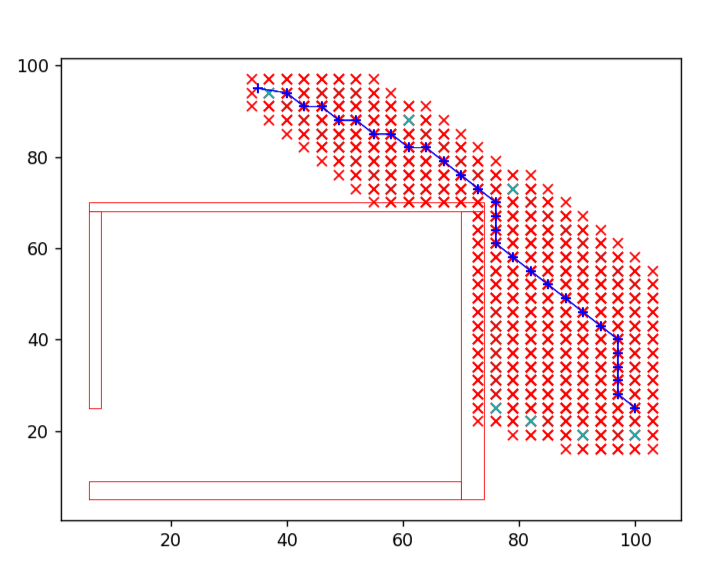
\includegraphics[width=0.6\textwidth]{A(star).png}
	\caption{A* node expansion showing exploration process}
	\label{fig:astar}
\end{figure}

The figure shows every cell visited during the search process, marked with red crosses. The algorithm successfully avoids the U-shaped trap in the center and reaches the goal, indicated by the blue star. This demonstrates the effectiveness of the heuristic function in guiding the search toward the goal while navigating around complex obstacles.

% ─── Step 2 ──────────────────────────────────────────────────────────────────
\subsection{Step 2: Generating the Raw Path}

Once the goal was found, the algorithm traced back through its steps to draw the route it had taken. This is called the raw path, shown as a green line in the figure.

Although this is technically right it takes over all the challenges and links the starting point to.
complete yet it is very rough. It consists of diagonal and right angle steps that are short.
follow the grid pattern of the map. A real robot cannot move in such a way: those sharp.
corners would make it come to a halt and turn and then come to a halt again each turn. So although
this is the step that the planner was sure that he has walked the correct path.
\begin{figure}[H]
	\centering
	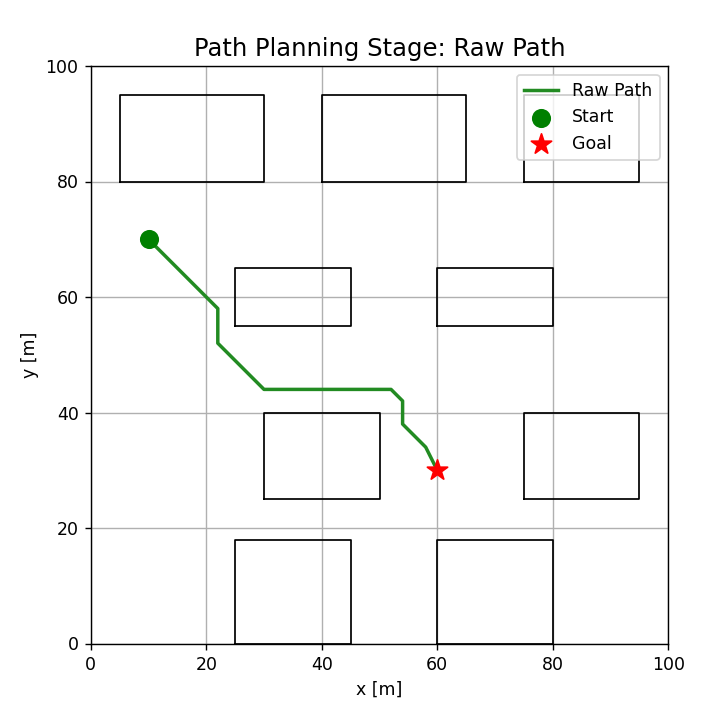
\includegraphics[width=0.7\textwidth]{Raw path.png}
	\caption{Raw path generated by A* algorithm}
	\label{fig:raw}
\end{figure}

The green line represents the raw path output from the A* algorithm. While collision free and connecting start to goal, the path follows the rigid grid structure, producing jagged movements with sharp corners. These movements are impractical for a real robot to execute smoothly, as they would require frequent stopping and rotation at each turn.

% ─── Step 3 ──────────────────────────────────────────────────────────────────
\subsection{Step 3: Cleaning Up the Path (Pruning)}

Then unnecessary waypoints were removed, making the trip easier. In order to ascertain whether it is possible to proceed straight ahead without running into any barriers, the trimming algorithm goes over the list of places. If this is the case, all intermediate points are removed because they are superfluous.

The outcome is a blue dashed line with much fewer points once the long, unnecessary zigzags are removed. This makes the robot's course more easier to follow and reduces the amount of computing needed later on.



\begin{figure}[H]
	\centering
	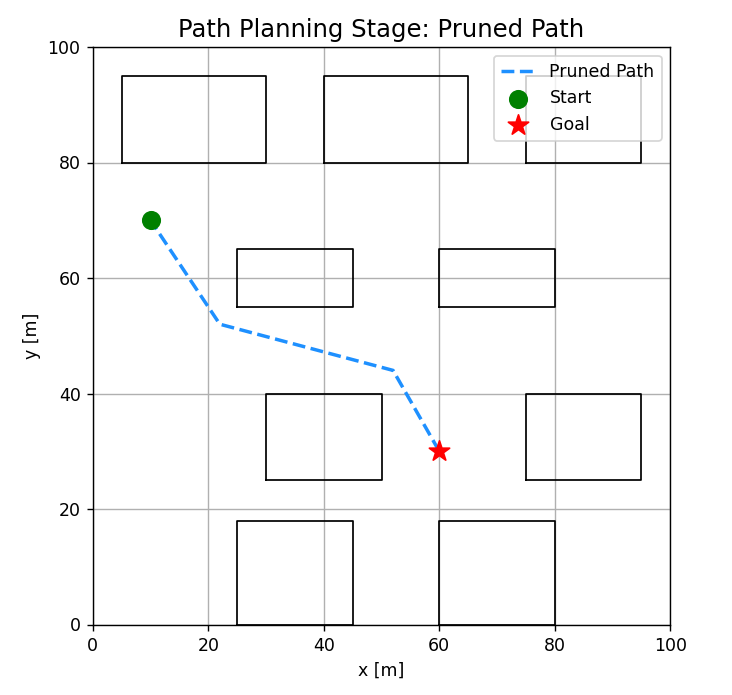
\includegraphics[width=0.7\textwidth]{pruned.png}
	\caption{Pruned path with redundant waypoints removed}
	\label{fig:pruned}
\end{figure}

The results of the pruning process are shown as a blue dashed line. Now the path is shorter and cleaner, due to the removal of redundant waypoints. This condensed path can be processed and followed much easier by the motion controller, which reduces the amount of computing resources required without compromising the obstacle avoidance.


% ─── Step 4 ──────────────────────────────────────────────────────────────────
\subsection{Step 4: Smoothing the Path}

All trimming methods resulted in the same ending, which was still a string of rectilinear segments, rounded at the corners. The last stage was to employ cubic spline interpolation to expertly integrate each of these components into a single continuous line.

The blue curving trajectory depicted in the illustration is the outcome. This arc-like trail is softer for the robot to follow than sharp bends. This is important as it means that a robot moving along a smooth curve can maintain a steady speed and not have to slow down for every turn. The smoothed trajectory is passed onto the following stage.


\begin{figure}[H]
	\centering
	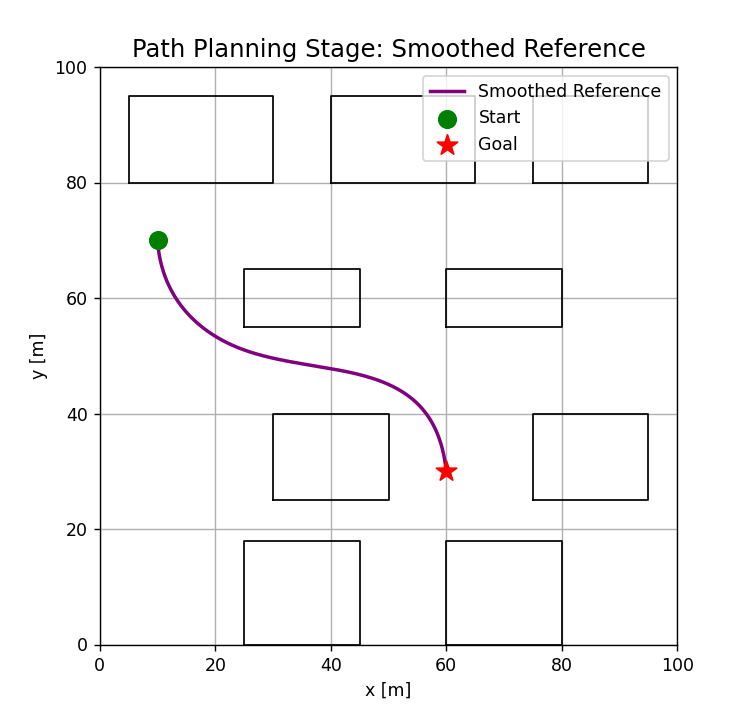
\includegraphics[width=0.7\textwidth]{smooth.png}
	\caption{Final smoothed trajectory using cubic spline interpolation}
	\label{fig:smooth}
\end{figure}

The blue curve is the final curve obtained by doing cubic spline interpolation. The road is now a continuous stream and is curved, with no sharp corners. This enables the robot to move without stopping at any turn, without slowing down during the trip, and will give smoother, more efficient motion.
% ══════════════════════════════════════════════════════════════════════════════
\section{Phase 2: Motion Control with MPC}

A Model Predictive Controller (MPC) was employed to enable the robot to accurately follow the generated reference path.

MPC looks ahead, which is the main distinction between it and a more straightforward controller like PID. It employs a short-term prediction of where the robot will be over the next few steps and modifies its motions accordingly, rather than only responding to where the robot is right now. Because it may begin slowing down or changing direction prior to a turn rather than after it has already missed it, this greatly improves its ability to handle curves.


The MPC was first implemented using a simple model of the robot, which
made it easier to test and tune the controller's core tracking behaviour. Once this
was working well, the MPC was reimplemented using the actual TurtleBot3 kinematic
model, so the controller respected the robot's real velocity limits and motion
constraints. All later tracking tests, including those in Gazebo, use this
TurtleBot3-based version of the MPC.% ─── Basic Test ──────────────────────────────────────────────────────────────
\subsection{Basic Tracking Test}

The blue line indicates the intended reference trajectory whereas the orange line indicates the real path taken by the robot. These two curves are nearly intersecting, which indicates that the controller had high level of precision at the beginning.

The plots on the right hand side illustrate the velocity and acceleration of the robot throughout the period of time in the experiment. The robot has these profiles and no unstable excursions or sharp spikes in the profiles that would indicate that the robot ran in an unexpected manner or impediment was encountered during the run which would have caused these spikes.

\begin{figure}[H]
	\centering
	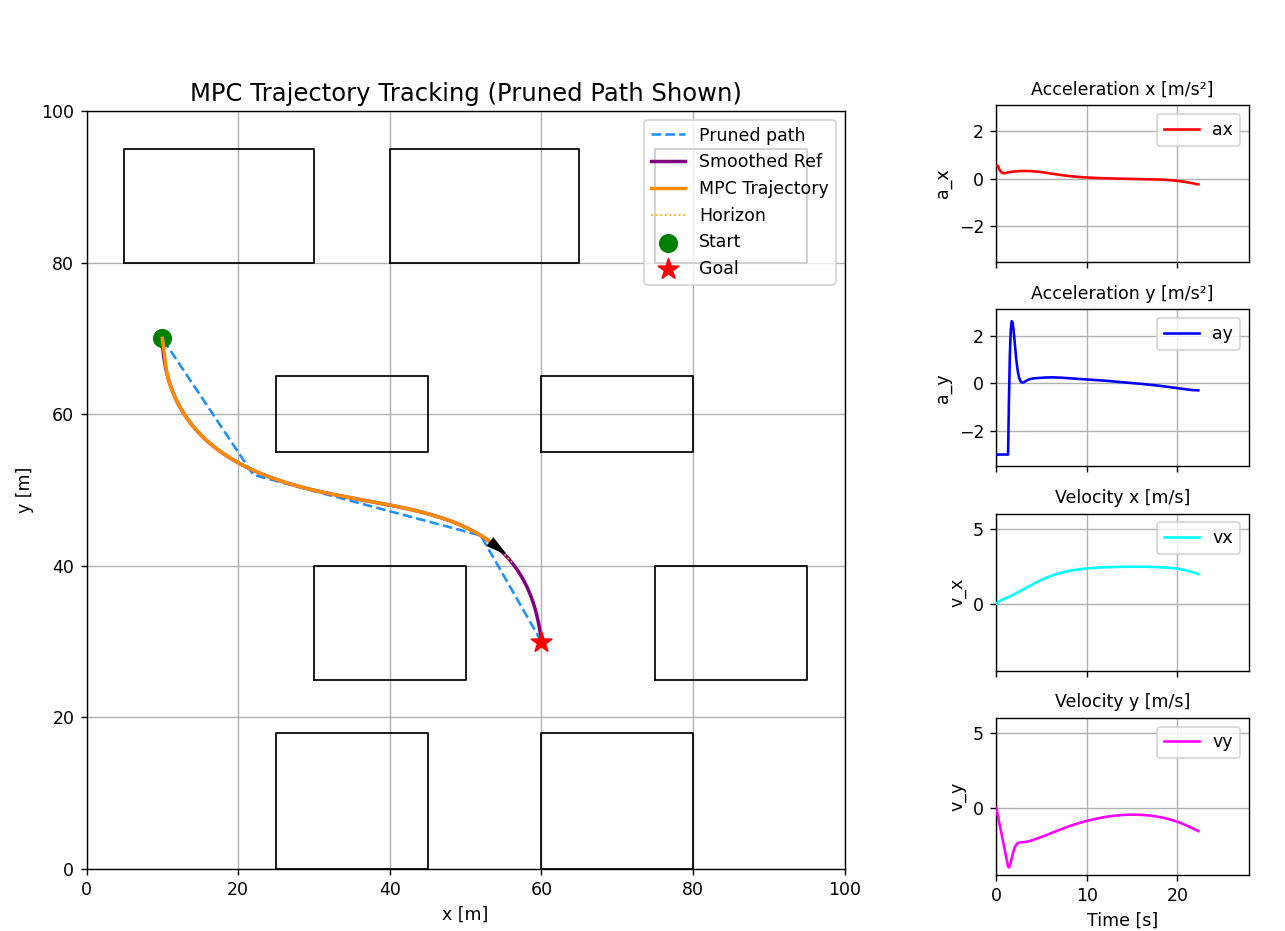
\includegraphics[width=0.85\textwidth]{MPC 1.png}
	\caption{MPC tracking test results}
	\label{fig:mpc1}
\end{figure}

The figure collectively depicts the MPC controller's tracking performance. The orange curve matches the purple curve along the reference path's side plots over the entire time span, with smooth velocity/acceleration plots indicating controlled, inconspicuous motion by the robot without abrupt and erratic transitions.


% ─── Dual Scenario ───────────────────────────────────────────────────────────
\subsection{Testing in Two Different Environments at Once}

The controller was tested in a maze with very small corridors (Scenario~1) and in a large open space (Scenario~2), to ensure that it does not just work very well in one specific map. This comparison against the side was useful in establishing not only the MPC's tuning to a specific configuration, but also as a means of establishing reliability.


\subsubsection{Start of the Mission}

The robot (green dot) is at the start of its path in each map. The orange dotted line extending forward shows the controller's short-term prediction the window of future movement it is planning for at any given moment. Both environments loaded correctly and the MPC was ready to begin tracking.

\begin{figure}[H]
	\centering
	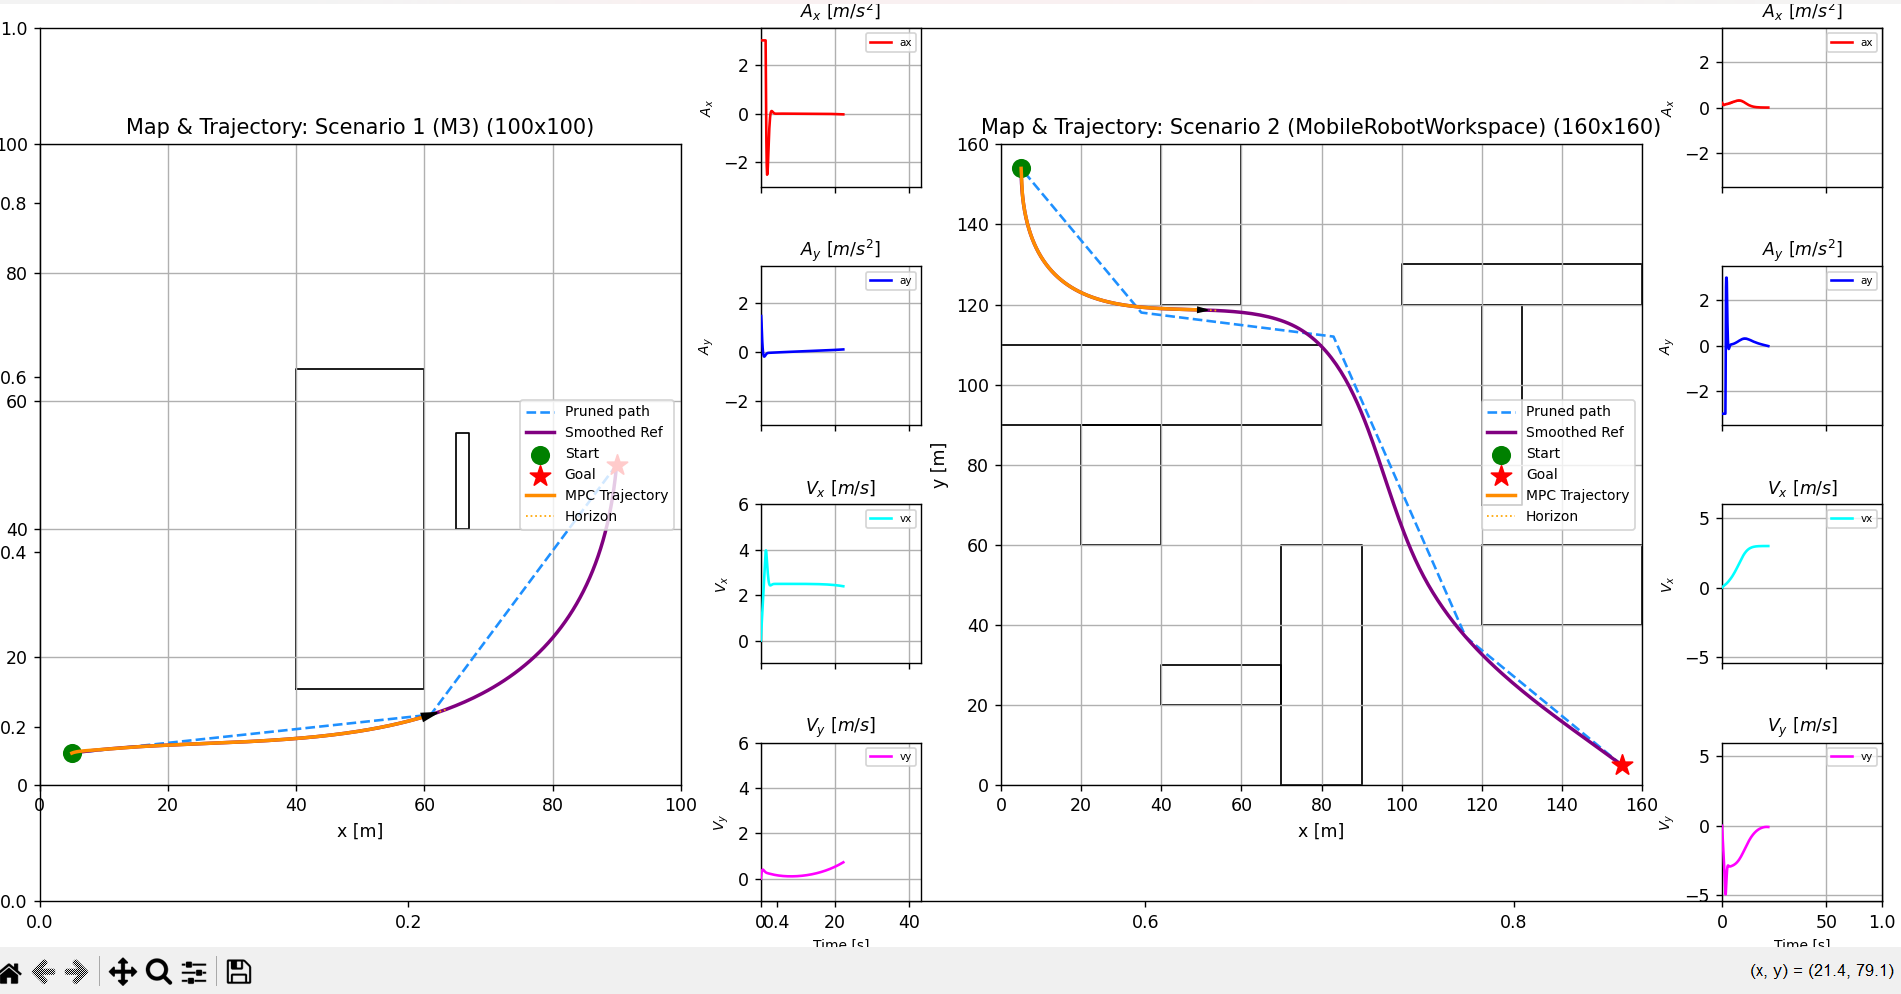
\includegraphics[width=0.9\textwidth]{MPC(start).png}
	\caption{Both environments at mission start}
	\label{fig:mpc_start}
\end{figure}

The figure shows both test environments at the beginning of the mission. The green dot represents the robot's starting position in each scenario. The orange dotted line extending forward illustrates the MPC's lookahead prediction horizon, showing the short-term future movement window that the controller is actively planning for at this instant.

\subsubsection{End of the Mission}

Once both runs completed, the orange path the robot actually took falls almost perfectly on top of the planned purple path in both maps. Whether navigating tight corners in the maze or covering a large open distance, the controller maintained the same level of accuracy throughout confirming the system is not sensitive to map layout.

\begin{figure}[H]
	\centering
	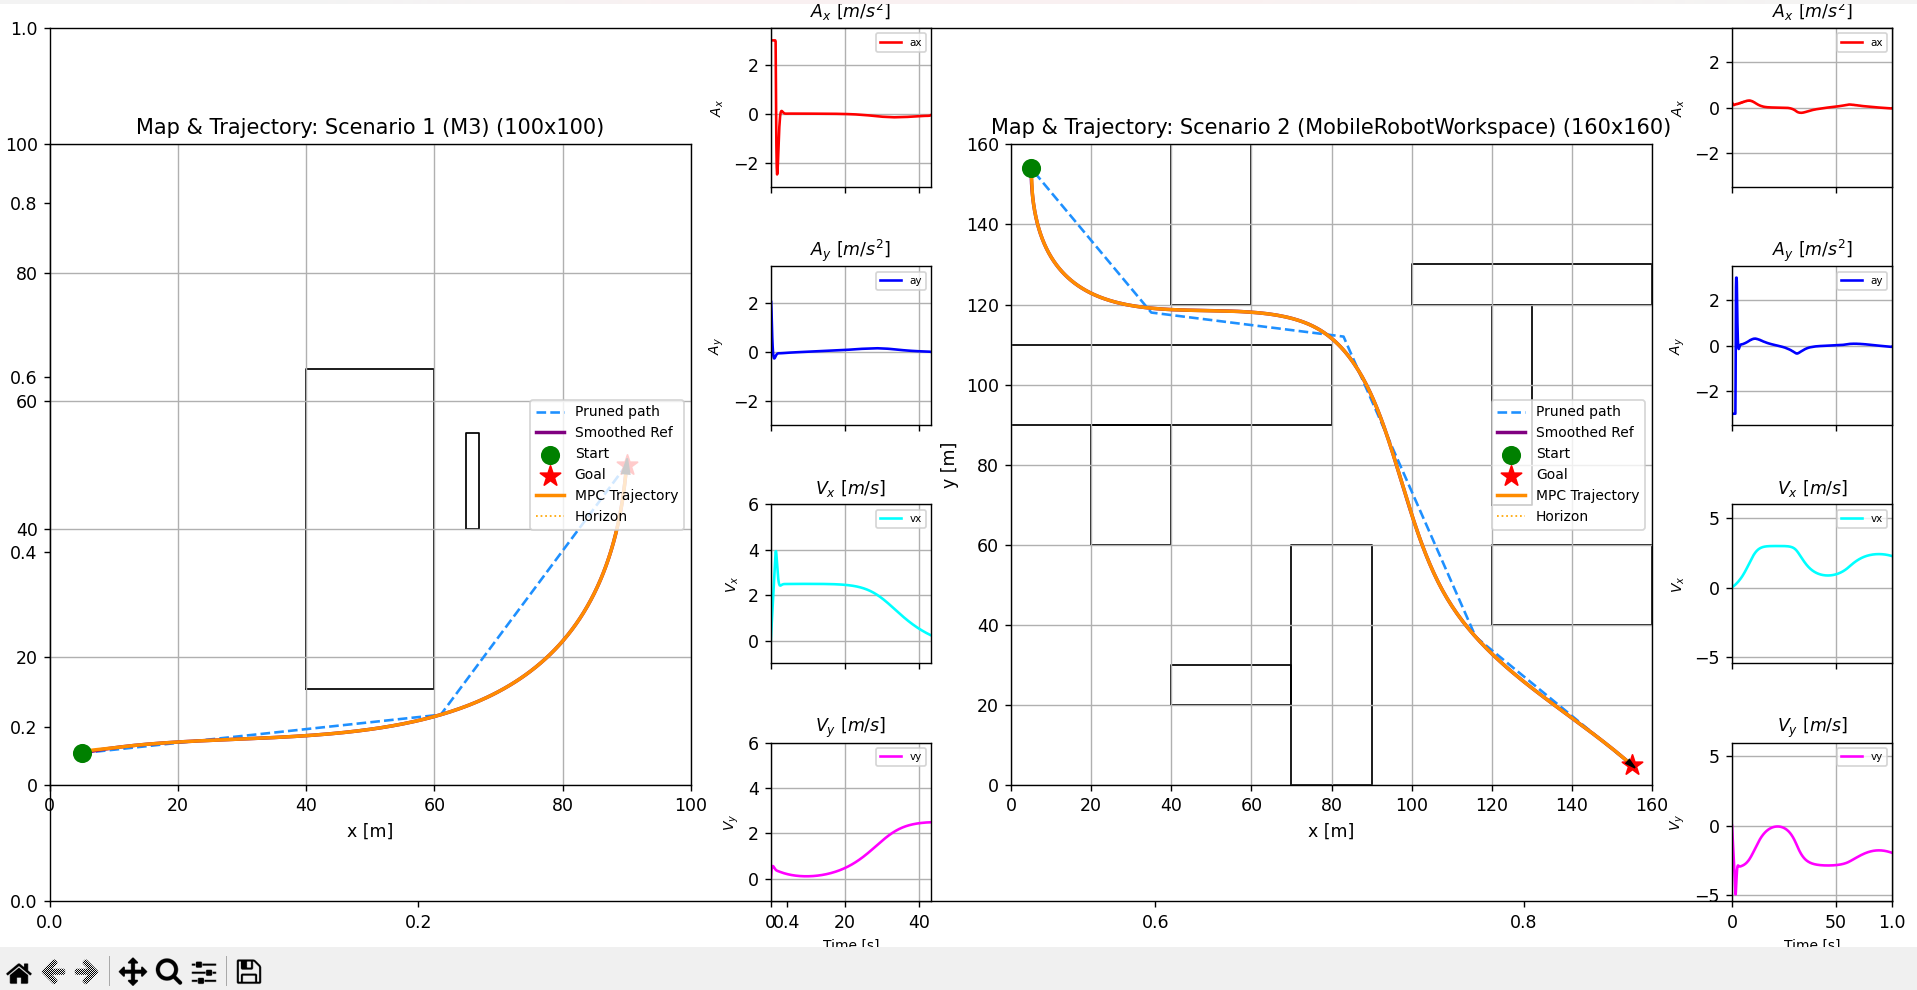
\includegraphics[width=0.9\textwidth]{MPC(end).png}
	\caption{Both environments at goal convergence}
	\label{fig:mpc_end}
\end{figure}

The successful completion of mission is shown in both environments, as seen in the image \ref{fig:mpc_end}. The orange real path is shown on top of the purple reference path in both cases, with consistent tracking accuracy in both cases, regardless of the complexity of the surroundings. The MPC controller does a good job in different map layouts and situations of navigation.


% ─── Error Analysis ──────────────────────────────────────────────────────────
\subsection{Measuring the Tracking Error}
While it can be useful to simply look at the paths, it is more useful to determine the actual error of the controller. In both cases, the deviation of the robot from the reference path (cross-track error) was observed at any time.


\subsubsection{Scenario 1: Standard Maze}

There is a slight increase in inaccuracy at the beginning of the run. The robot is accelerating from a standstill and briefly exceeding the speed before slowing down—typical. The inaccuracy decreases to almost zero after a few seconds. There are brief, little bumps throughout the maze's rapid curves, but they go away fast. The error was still significant when moving at constant speed (2~cm).


\begin{figure}[H]
	\centering
	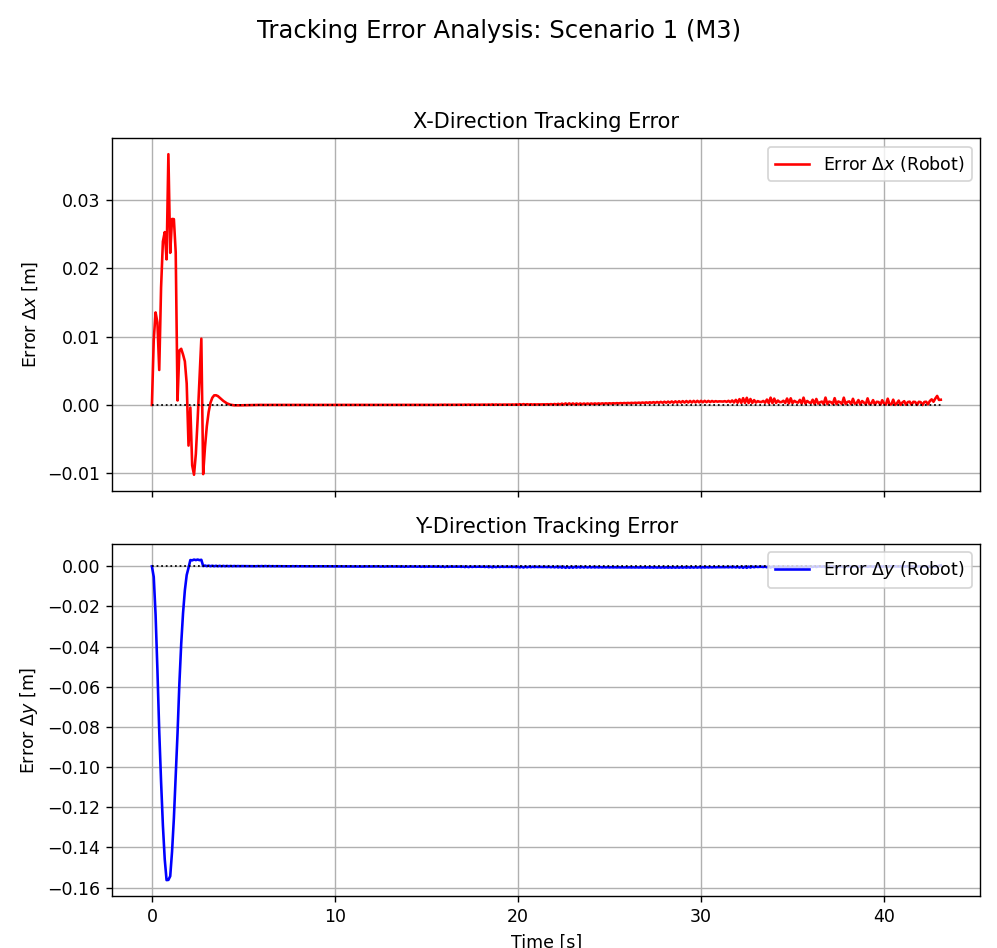
\includegraphics[width=0.85\textwidth]{Tracking Error Analysis S1.png}
	\caption{Tracking error analysis for Scenario 1}
	\label{fig:error_s1}
\end{figure}

The cross track error for the maze environment with time is shown in the figure. Inaccuracy quickly settles into almost a constant value after an initial transient upon startup and remains below 2~cm throughout the trip. Its ability to navigate tight corners with little error can be seen in the quick correction of the errors that occur at the corners.The controller's ability in difficult to navigate situations, with tight bends, is shown by the brief error spikes that occur at steep curves followed by quick corrections.


\subsubsection{Scenario 2: Large Open Workspace}

Compared to the maze, the open workspace yielded an even smoother error profile. The error signal was not fluctuating much during the bulk of the run and the amount of corrective action performed by the controller was less since there were fewer sharp corners to overcome. This shows the MPC to be capable and effective in less demanding situations and competent in more demanding situations.


\begin{figure}[H]
	\centering
	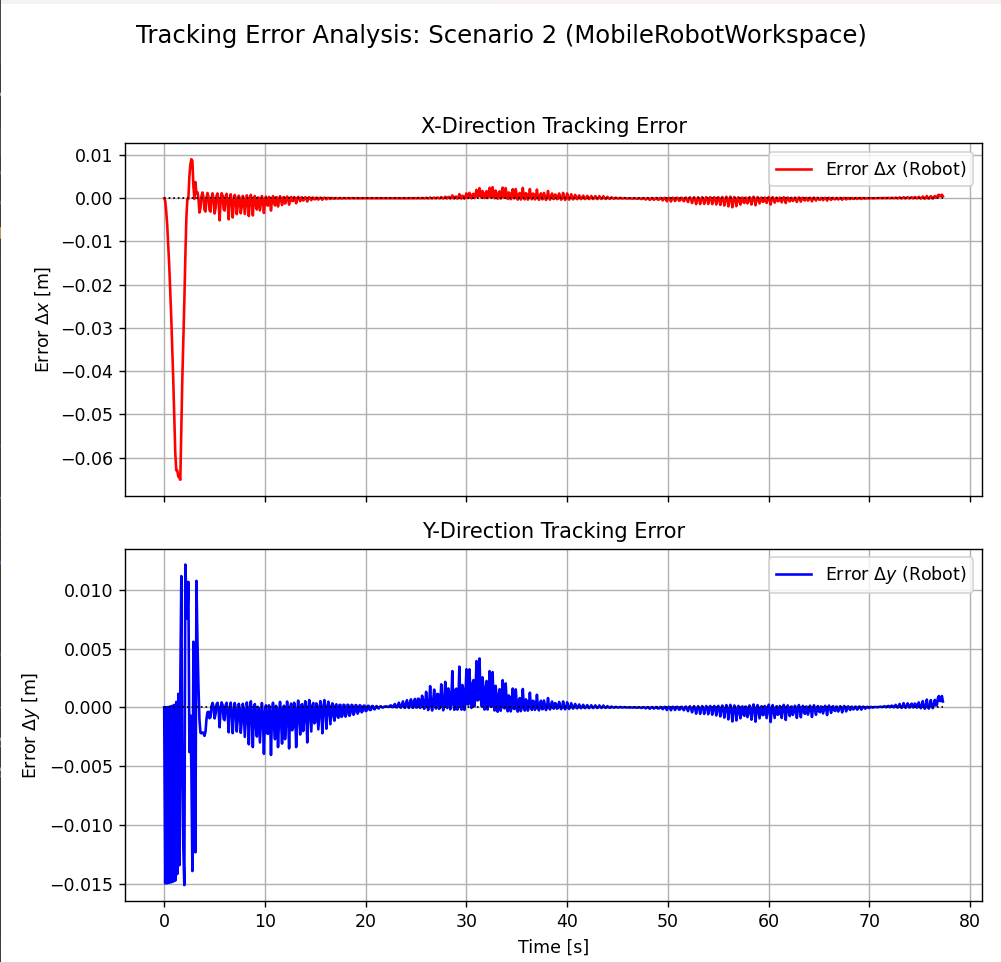
\includegraphics[width=0.85\textwidth]{Tracking Error Analysis S2.png}
	\caption{Tracking error analysis for Scenario 2}
	\label{fig:error_s2}
\end{figure}

The error profile in the open workspace will be quite flat as there are fewer requirements for curvature. The controller works better in regions with relatively few limits as it keeps the tracking error extremely small during the entire course of the mission in less challenging spaces with lesser sharp bends. 



% ─── Stress Test ─────────────────────────────────────────────────────────────
\subsection{Stress Test: Circles and Triangles}

To this end, a specially designed map with irregularly shaped obstacles in the form of triangles and circles has been constructed, in order to further test the motion controller. This led to very restricted and cumbersome routes. Because these non-orthogonal designs produce sharp angles and curved sides that call for quick and precise navigational maneuvers, they are more challenging to handle than the more conventional rectangular barriers.   

The little openings the robot navigated through weren't blocked and the bot didn't get confused.
Its path sensorimotor remained in a steady flow even as it manoeuvred around the sharp corners of triangular shapes hence proving that the Model Predictive Control scheme has the ability to cope with the challenging geometries just as easily as simpler ones.
\begin{figure}[H]
	\centering
	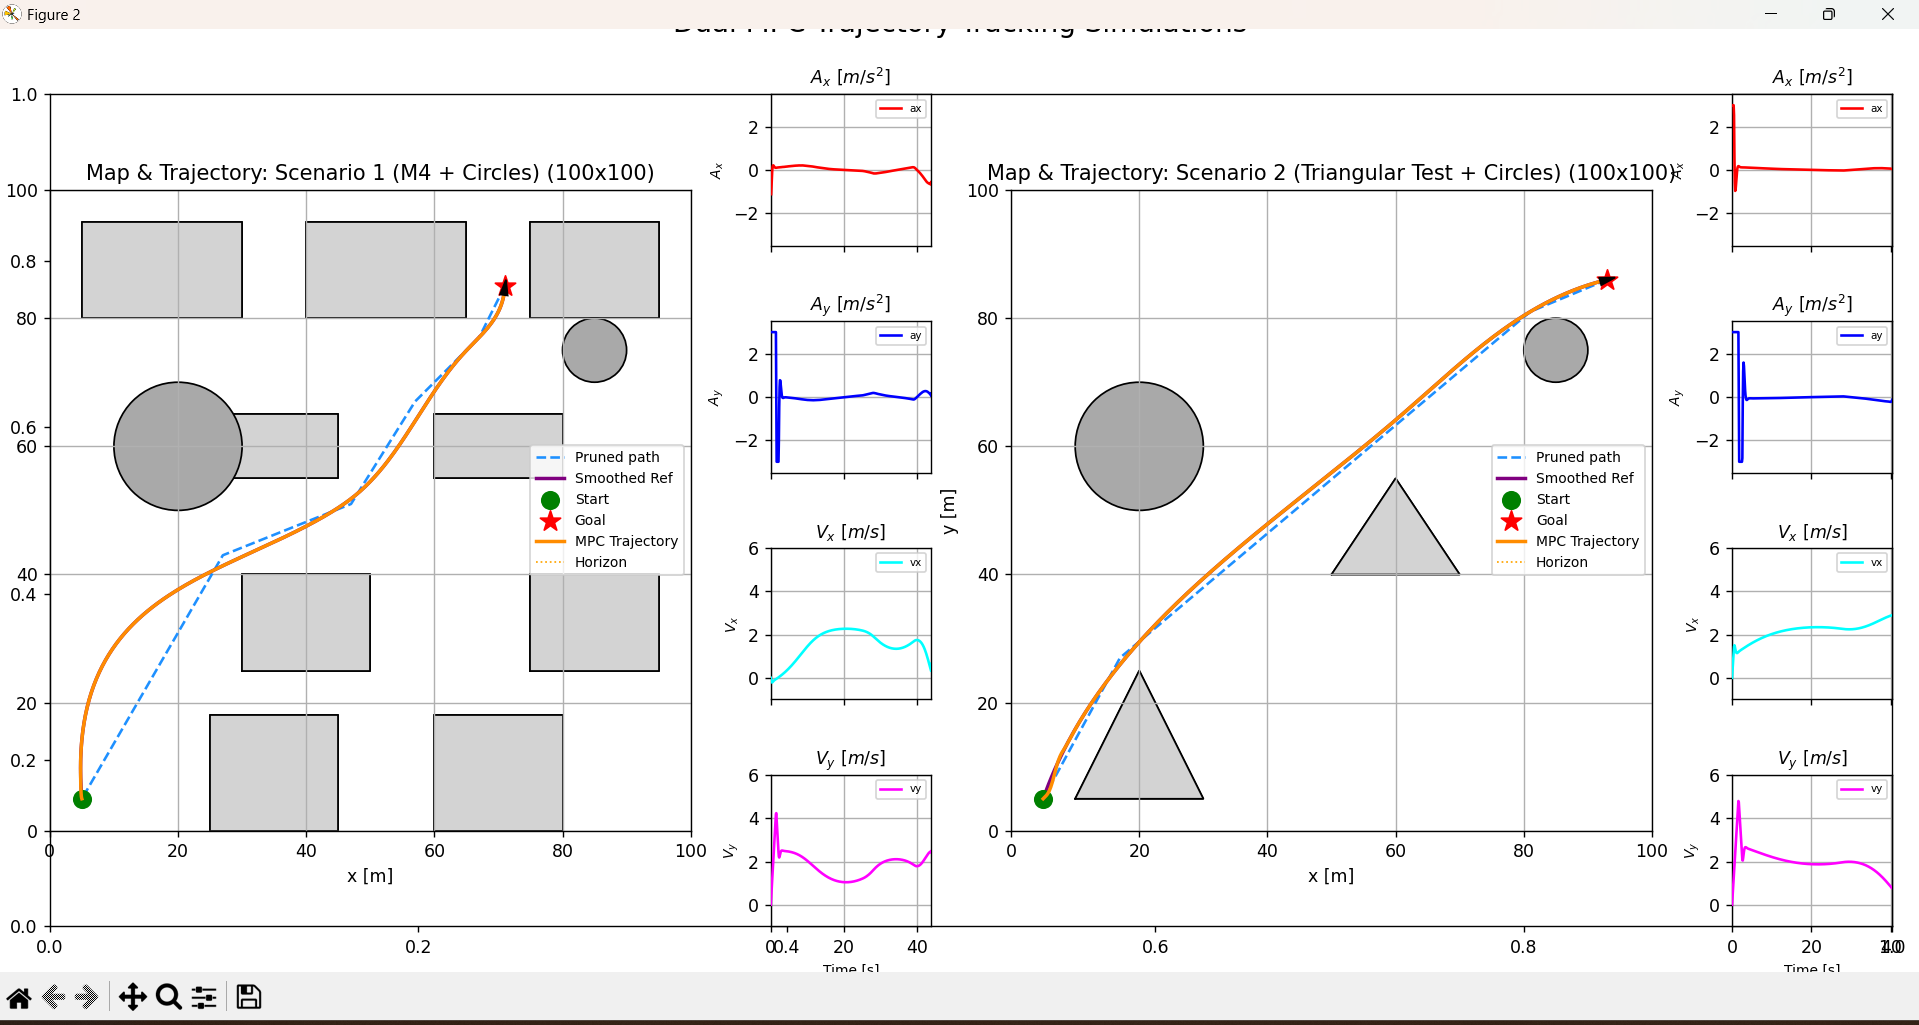
\includegraphics[width=0.85\textwidth]{MPC(Circle+triangle).png}
	\caption{Stress test with circular and triangular obstacles}
	\label{fig:mpc_complex}
\end{figure}

The controller's performance with complicated obstacle geometries is shown in figure \ref{fig:mpc_complex}. The robot maintains a smooth course while successfully navigating every narrow space between triangular and circular obstacles. This confirms that the MPC can manage complex geometric arrangements and unusual obstacle shapes that call for quick, accurate trajectory modifications.


\subsection{TurtleBot3 Model Tracking of PSO-Smoothed Path}

Dedicated tracking simulations were performed on both test maps using the TurtleBot3's motion parameters in order to confirm that the MPC controller could consistently track the PSO-smoothed path while adhering to the kinematic and velocity constraints of the real TurtleBot3 robot model. Each graphic displays the MPC trajectory superimposed on the same map as the trimmed A* path, the PSO control points, and the resulting PSO-smoothed path.


\subsubsection{Start of the Tracking Run}

Both possibilities are displayed at the start of the tracking run in Figure~\ref{fig:pso_mpc_start}.
The trimmed A* path (blue dashed line) in each map has previously been optimized into a smooth continuous trajectory (green line) and transformed into a set of PSO control points (orange squares). In both the compact map and the larger MobileRobotWorkspace map, the MPC trajectory (solid orange line) produced by the TurtleBot3 kinematic model is just starting to follow this smoothed reference from the start position (green dot) toward the goal (red star). As the controller begins tracking while staying within the TurtleBot3's operational parameters, the side plots display the initial acceleration and velocity response.


\begin{figure}[H]
	\centering
	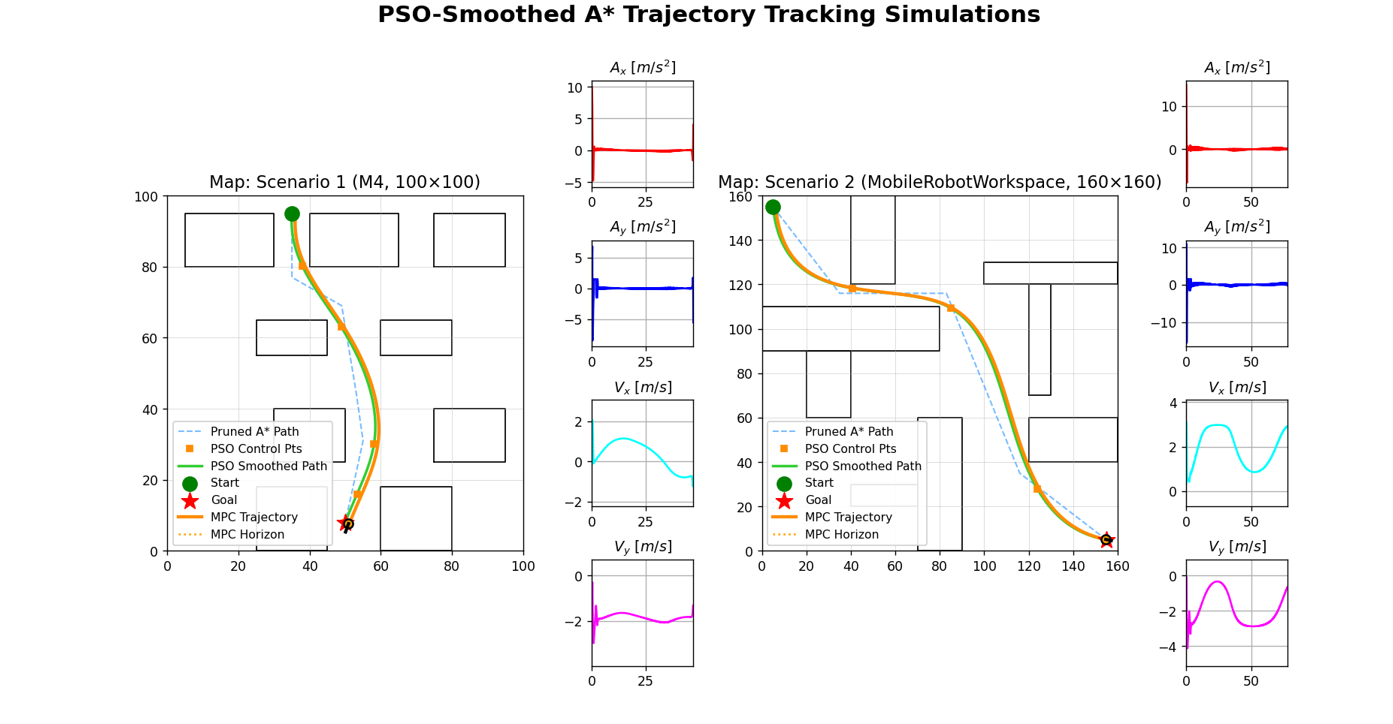
\includegraphics[width=1\textwidth]{pso_mpc_tracking_start.png}
	\caption{TurtleBot3 Model MPC Tracking of the PSO-Smoothed A* Trajectory at the Start of the Mission}
	\label{fig:pso_mpc_start}
\end{figure}

\subsubsection{End of the Tracking Run}

Both scenarios are displayed at the end of the tracking run in Figure~\ref{fig:pso_mpc_end}.
Now that the MPC trajectory has successfully reached the goal location in each scenario, it nearly perfectly covers the whole length of the PSO-smoothed path in both maps. The controller maintained steady, low-jerk motion compatible with the TurtleBot3's kinematic limitations from beginning to end, as seen by the acceleration and velocity profiles remaining smooth throughout.


\begin{figure}[H]
	\centering
	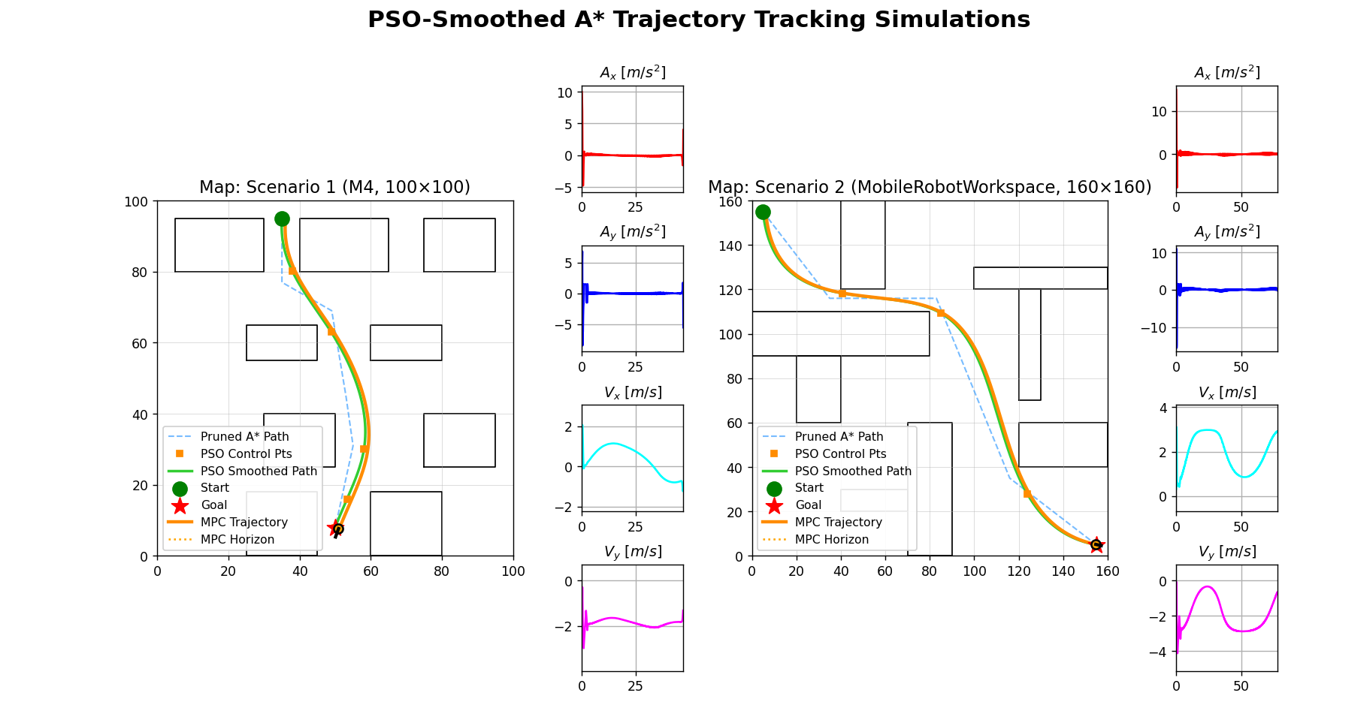
\includegraphics[width=1\textwidth]{pso_mpc_tracking_end.png}
	\caption{TurtleBot3 Model MPC Tracking of the PSO-Smoothed A* Trajectory at the End of the Mission}
	\label{fig:pso_mpc_end}
\end{figure}

These findings verify that, regardless of map size or obstacle layout, the MPC controller, set up with the TurtleBot3's kinematic model, precisely tracks the PSO-smoothed reference path from start to goal, generating smooth, low-jerk motion profiles consistent with the robot's real-world motion capabilities.


\subsection{Keeping the Robot Safe: Obstacle Inflation}
One crucial safety feature that is integrated into the navigation backend is obstacle inflation. The algorithm is used not on the physical obstacle itself, but on a mathematical expansion of the footprint of the obstacle, which forms a virtual "no-go" buffer zone.


Figure \ref{fig:inflation} visualizes this mechanism clearly. The diagram differentiates between two distinct zones:
\begin{itemize}
	\item \textbf{Original Obstacle:} 
	The core area is light pink and is used to indicate what the object physically would look like.
	
	\item \textbf{Inflated Obstacle:} 
	The outer drawing is the safety buffer as drawn by the algorithm and is drawn in deeper red.
\end{itemize}

Hard limit is the Inflated edge, the path planner is forced to keep distance to the physical object (the robot). This essentially supplies the uncertainties encountered in the real world, such as sensor noise, or small localization errors, and thus the robot (initially in the green marker) will never hit the wall when working towards the goal (red square).



\begin{figure}[H]
	\centering
	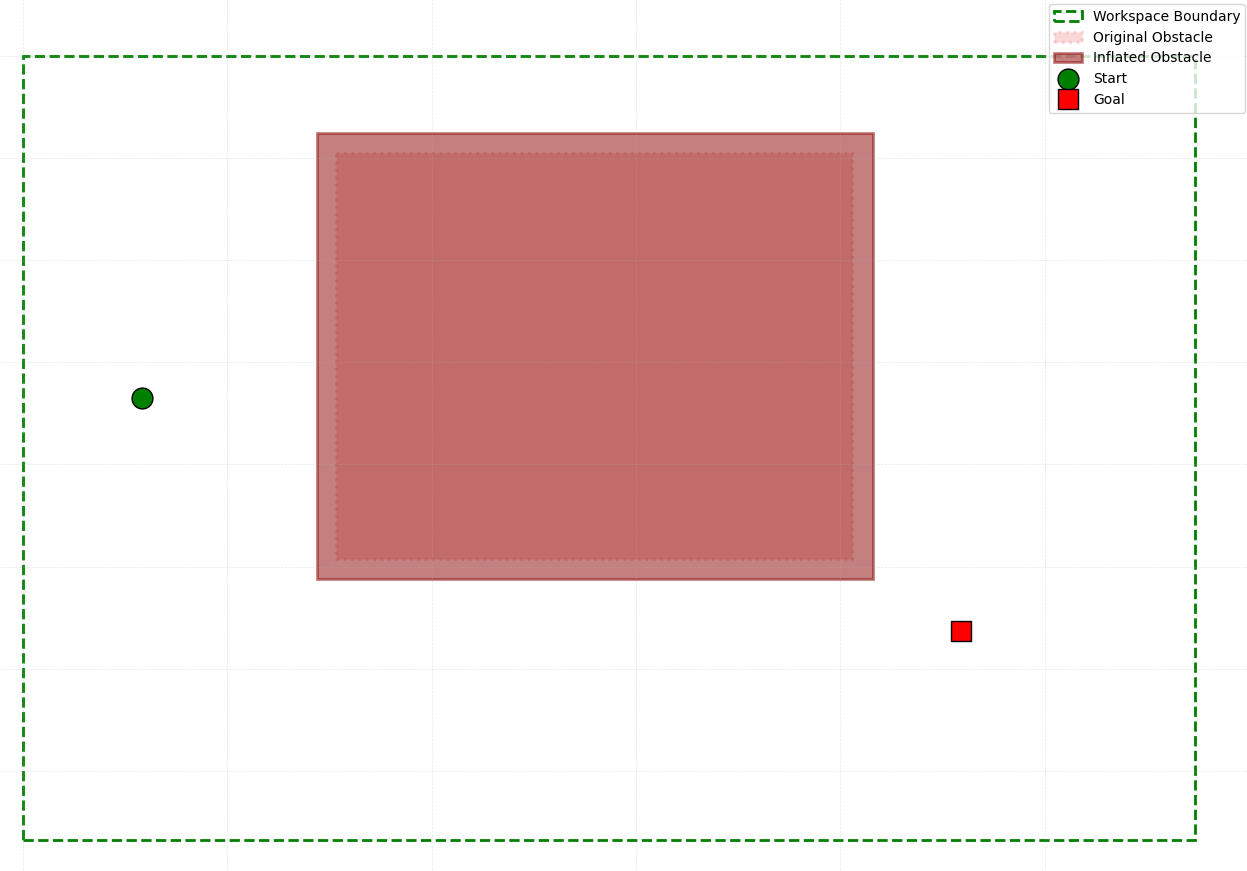
\includegraphics[width=0.8\textwidth]{inflation.png} 
	\caption{Obstacle inflation}
	\label{fig:inflation}
\end{figure}

% ══════════════════════════════════════════════════════════════════════════════
\section{Phase 3: Web Interface}

When the basic algorithms were successful, a web-based control interface was created to enable a person to observe the robot and set the delivery tasks without any code or ROS~2. Making the system usable by everyone, not just technical experts, was the aim.


% ─── Dashboard ───────────────────────────────────────────────────────────────
\subsection{The Control Dashboard}

A particular interface for mission planning is the control dashboard. The system will ultimately be able to accept custom facility maps or Point Cloud Data (PCD), but for the purposes of this demonstration it is based on an OpenStreetMap layer to provide a realistic visual context.

The interface follows a structured, step-by-step workflow to ensure secure path generation:
\begin{enumerate}
	\item \textbf{Define Workspace:} To define the robot's safe working area, the operator first chooses the "Draw Boundary" option.

	\item \textbf{Place Obstacles:} Next, users can draw virtual obstacles (using Rectangle or Circle tools) to represent restricted zones, such as construction areas or temporary hazards.
	\item \textbf{Assign Mission:} Finally, the operator marks the exact Start point (Green Marker) and End point (Red Marker) which characterize the delivery task.
	
\end{enumerate}
When this configuration is accomplished, the static map information is fed into the backend computational routines and the optimal trajectory is calculated. This configuration based architecture will enable non-technical staff to gain the ability to conduct safe and effective designation of the environment the robot will operate in, before implementation.
\begin{figure}[H]
	\centering
	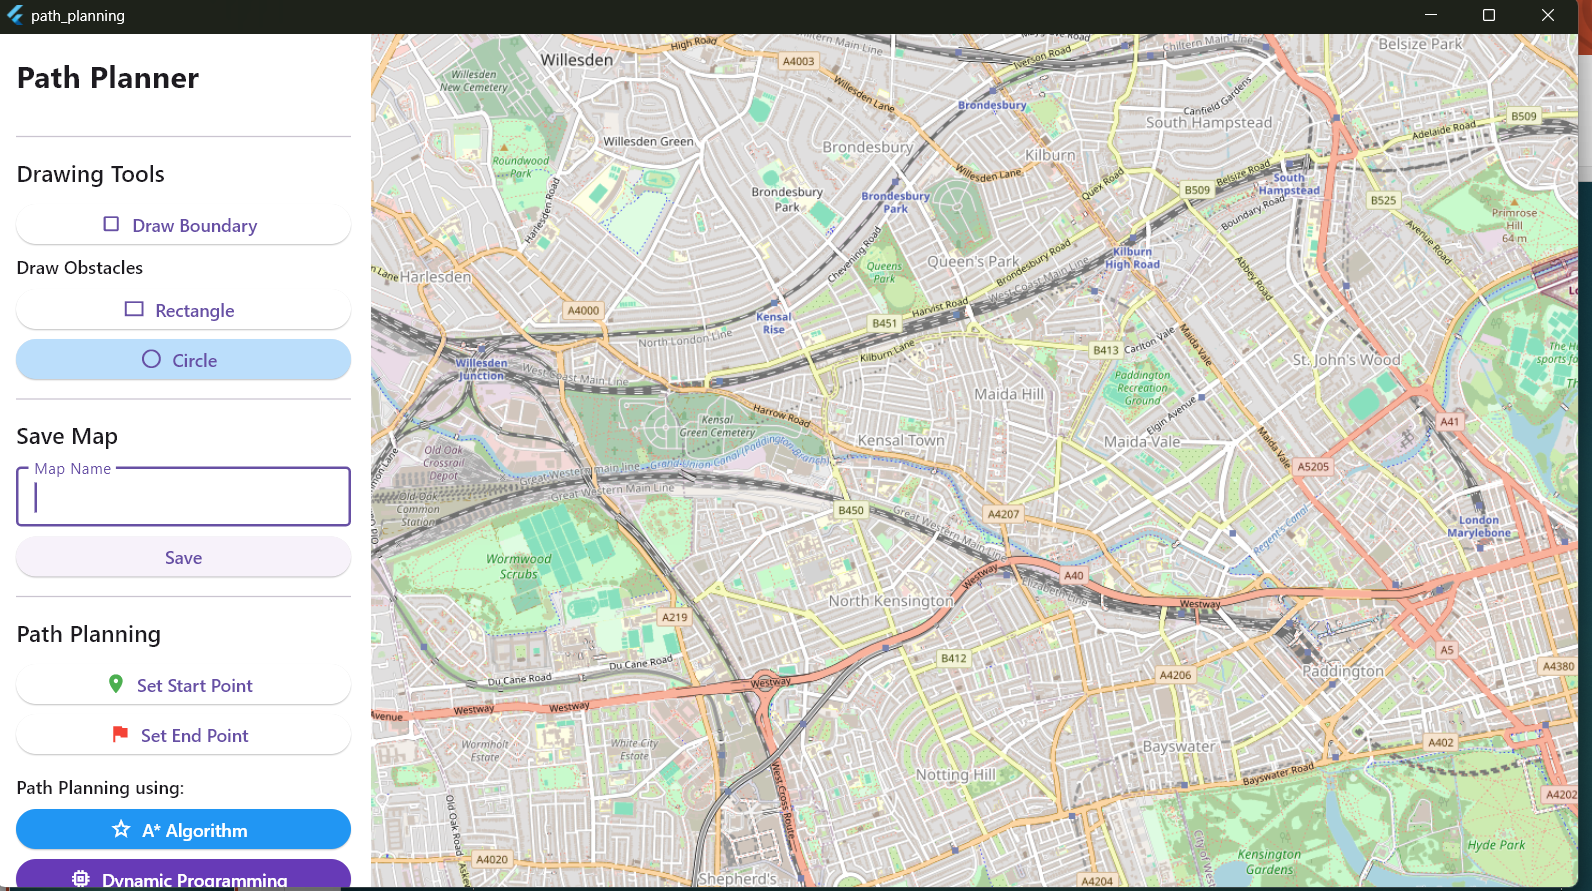
\includegraphics[width=0.95\textwidth]{webapp.png}
	\caption{Web control dashboard used for defining boundaries, obstacles, and mission points}
	\label{fig:webapp}
\end{figure}
% ─── Inflation ───────────────────────────────────────────────────────────────
\section{2D Global Planner Results}

We ran the global planner on the 2D map environment first before entering the full 3D simulation. The aim of those tests was ensuring that the planner is capable of producing safe and correct paths in varying obstacle layouts. A 2D version allows us to exercise sanity of the path planning code without wasting time on robot dynamics, sensor noise or real-time control issues.

In order to assess the planner correctly we established three scenarios. Each scenario was tailored to test a unique factor, one that entailed obstacle avoidance with an adequate safety margin, one to avoid blocking obstacles, and the final was to plan distances on a larger scale on a cluttered map.
\subsection{Cellular Decomposition Output (2D Workspace Partitioning)}
In order to make global navigation in a complex indoor setting simple, we adopted a cellular decomposition method on the 2D workspace. The primary aim of this step is to divides into several non-overlapping areas (cells) the free space according to the boundaries of obstacles. The cells are safe zones where the robot will not run into anything.

Once the cells are decomposed, A representative point (cell center) is chosen for each region. These centers are then used to build an adjacency graph of connectivity.This graph helps the planner to easily determine a possible route from start to finish, and provides a simplified, high level structure of the environment.


Figure~\ref{fig:cellular_decomposition} shows the final output of the cellular decomposition
process, including the generated cells, their connectivity, and the resulting global path.
The planned route demonstrates how the robot transitions between cells while avoiding
obstacles and restricted regions.

\begin{figure}[H]
	\centering
	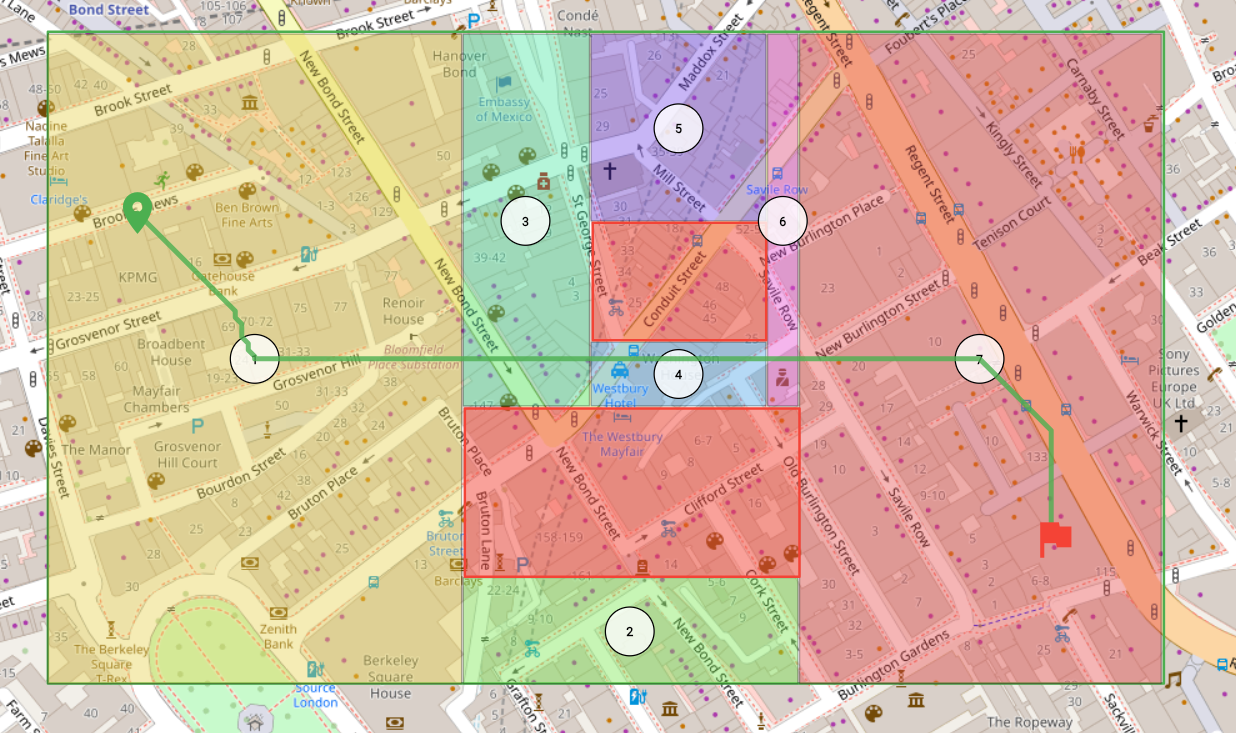
\includegraphics[width=0.8\textwidth]{grid.png}
	\caption{Output of cellular decomposition showing workspace partitioning into cells,
		adjacency connectivity, and the generated global path from start to goal.}
	\label{fig:cellular_decomposition}
\end{figure}


\subsection{Scenario A: Path Planning with Obstacle Avoidance}

In the first test (Figure \ref{fig:scen1}), the planner was given a task to navigate from the start point to the goal while avoiding a large circular restricted zone.The main factor when planning the robotic paths would be the definition of the workspace boundary, which defines the allowed area of operation. The robot has the responsibility of seeing that he does not cross this line, and at the same time, keeps to a predetermined safe distance of any possible dangers.

The importance of the given test is that it allows assessing the skills of the planner in coping with obstacle inflation. The test environment has a circular obstacle surrounding which has been superimposed a safety buffer, a light pink annulus in which is placed a darker core. The planner must be able to make certain that the trajectory of the robot does not trespass on this inflated area, but only avoids the physical limit of the obstacle.

Experimental findings suggest that the planner found a smooth curvy path and was able to maneuver through the obstacle and maintain the necessary clearance distances. Notably, the route does not violate the workspace limitations and infringe upon the limited area, which proves the effectiveness of the adopted safety margin system.

\begin{figure}[H]
	\centering
	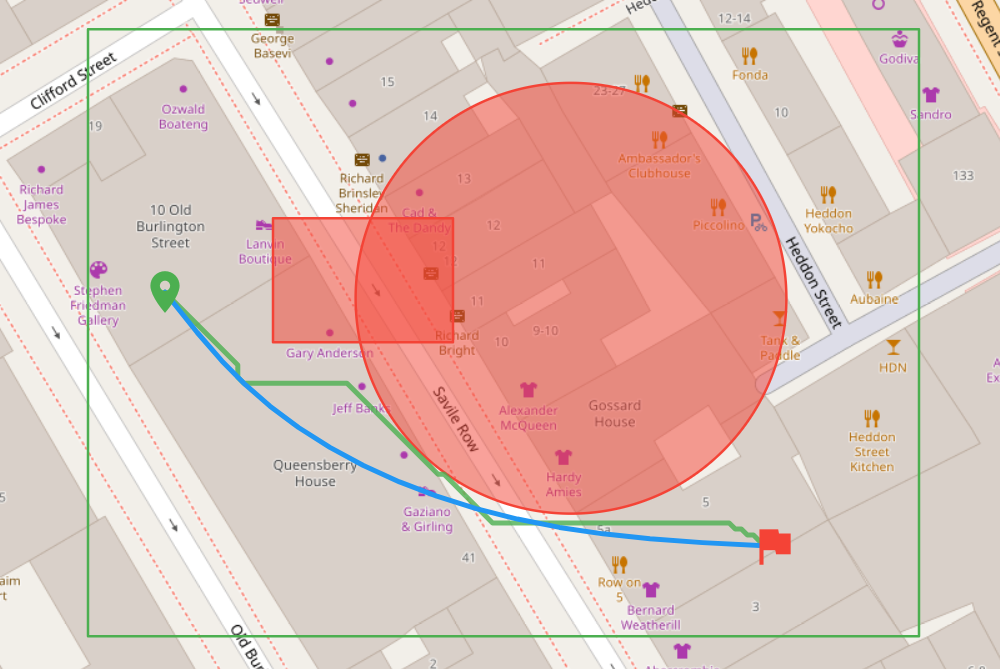
\includegraphics[width=0.7\textwidth]{test2.png}
	\caption{Scenario A: Path planning with obstacle avoidance}
	\label{fig:scen1}
\end{figure}
The findings reveal that the planner was able to find a smooth and curved path that bypasses the obstacle maintaining sufficient clearance. The path also does not go too far in the spatial boundaries of the working area and does not go too close to the limited area. This makes the efficacy of the safety margin system confirmed by these observations.

\subsection{Scenario B: Navigating Around Multiple Obstacles}

The second test (Figure \ref{fig:scen2}) included both a large circular obstacle and a rectangular restricted zone.
The rounded barrier was placed in such a manner that it was on the most direct path of the initial and final destinations forcing the planner to come up with an alternative path.

This scenario will analyse the ability of the planner to solve the cases where straight line path is not possible. In the operational delivery situations, furniture, equipment, or provisional barriers often hinder the shortest path; therefore the robot has to be intelligent enough to avoid these obstacles.

The outcomes prove that the planner generated a smooth detour by which the circular obstacle was circumscribed and the rectangular zone was avoided at the same time. The path experiences a natural curvature towards the obstruction and manages to hit the goal without any accidents.

These results can be attributed to the flexibility of the planner, who restructured the ways in the wake of hindering impediments.

\begin{figure}[H]
	\centering
	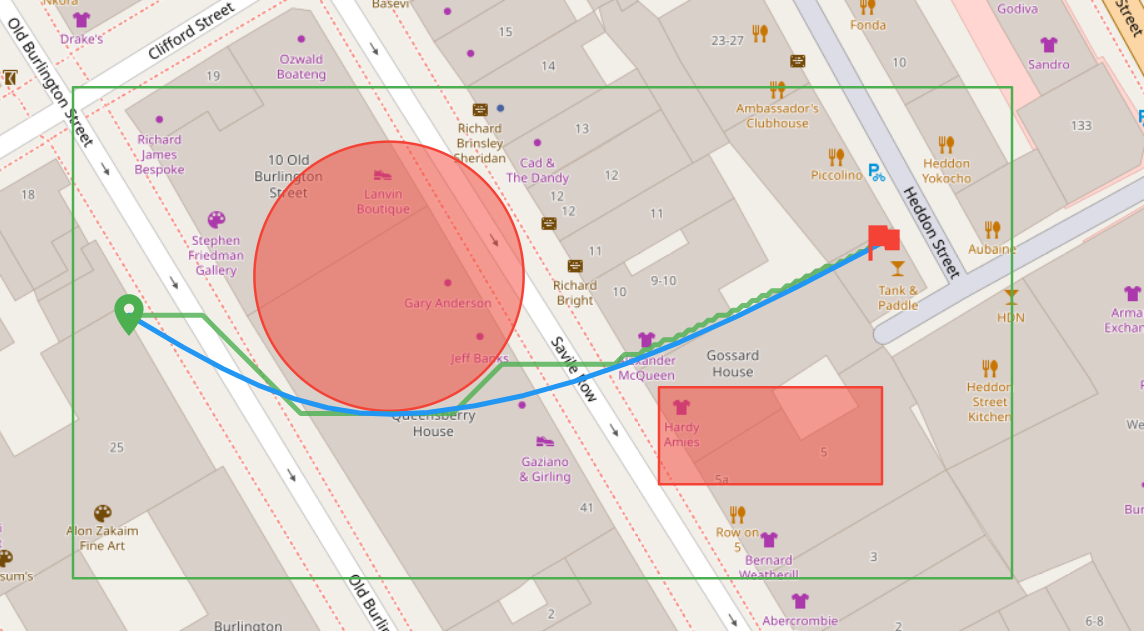
\includegraphics[width=0.7\textwidth]{test3.png}
	\caption{Scenario B: Navigating Around Multiple Obstacles}
	\label{fig:scen2}
\end{figure}

\subsection{Scenario C: Non-Convex Obstacle Negotiation}

The final test (Figure \ref{fig:scen3}) was designed to represent a more realistic delivery scenario.The area of workspace has been extended and a heterogeneous array of obstacles which has different geometry and dimension has been intentionally inoculated into the domain. The robotic platform therefore needs to move through a geodesic that is more significant in distance between its starting point and final goal, but at the same time having to manoeuvre through the ever growing cluttered environment.

This construct is used as a testbed, which is purposive, thus allowing an assessment of the soundness of the planner with respect to dimensional scalability and obstacle density. As the environmental topology continues to add more complexities, some planning methodologies can have a latency increment or worse still, fail to produce a viable answer.

The results of the empirical study confirm that the global planning module has managed to outline a continuous path between the source and the destination. The resulting trajectory sinuously navigates the landscape of forbidden areas, and always maintains the recommended buffer areas in relation to all the barriers it passes. The planner has therefore exhibited strength in increased complexity, and has been able to complete the mission within a reasonable time frame.
\begin{figure}[H]
	\centering
	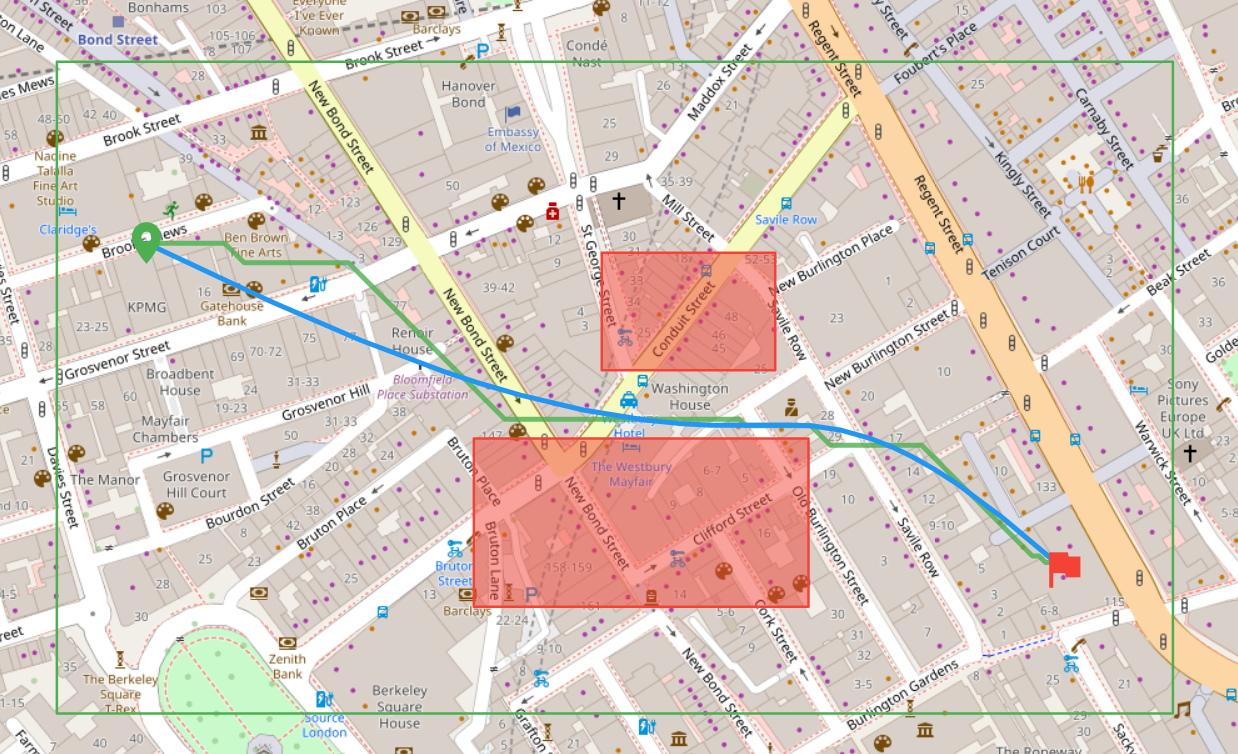
\includegraphics[width=0.7\textwidth]{test4.png}
	\caption{Scenario C: Long-range global planning across a multi-obstacle environment.}
	\label{fig:scen3}
\end{figure}

\subsection{Overall Observation}
In all of these three tests the planner is seen to be working extremely well in a range of two dimensional situations. It skillfully avoids obstacles with keeping the safety margins required, finds effective paths in case the current one is blocked, and moves on to larger and more complicated maps without any degradation.

Results act as confidence measures for the proper functioning of the path-planning algorithm even prior to the addition of the complexity of three-dimensional simulation. The planner will be tested in the ROS 2 and Gazebo settings in the next phase dynamic obstacles will be introduced.

\section{Phase 4: Flutter Web Application for Delivery Management}

While the dashboard described in Section 5.3 was used early in the project to validate map-based path planning, the delivery task itself is issued and monitored in practice through a dedicated Flutter web application built for end users, dispatch staff, and system administrators. The following section show the various screens of that application, including user authentication, requests for delivery, floor plan selection (with interaction), and administration tools for editing the facility map.

\subsection{Starting screen and Authentication}

The web starts with a simple presentation page showing a brief description of the system and its purpose before leading the user to the authentication interface.


\begin{figure}[H]
	\centering
	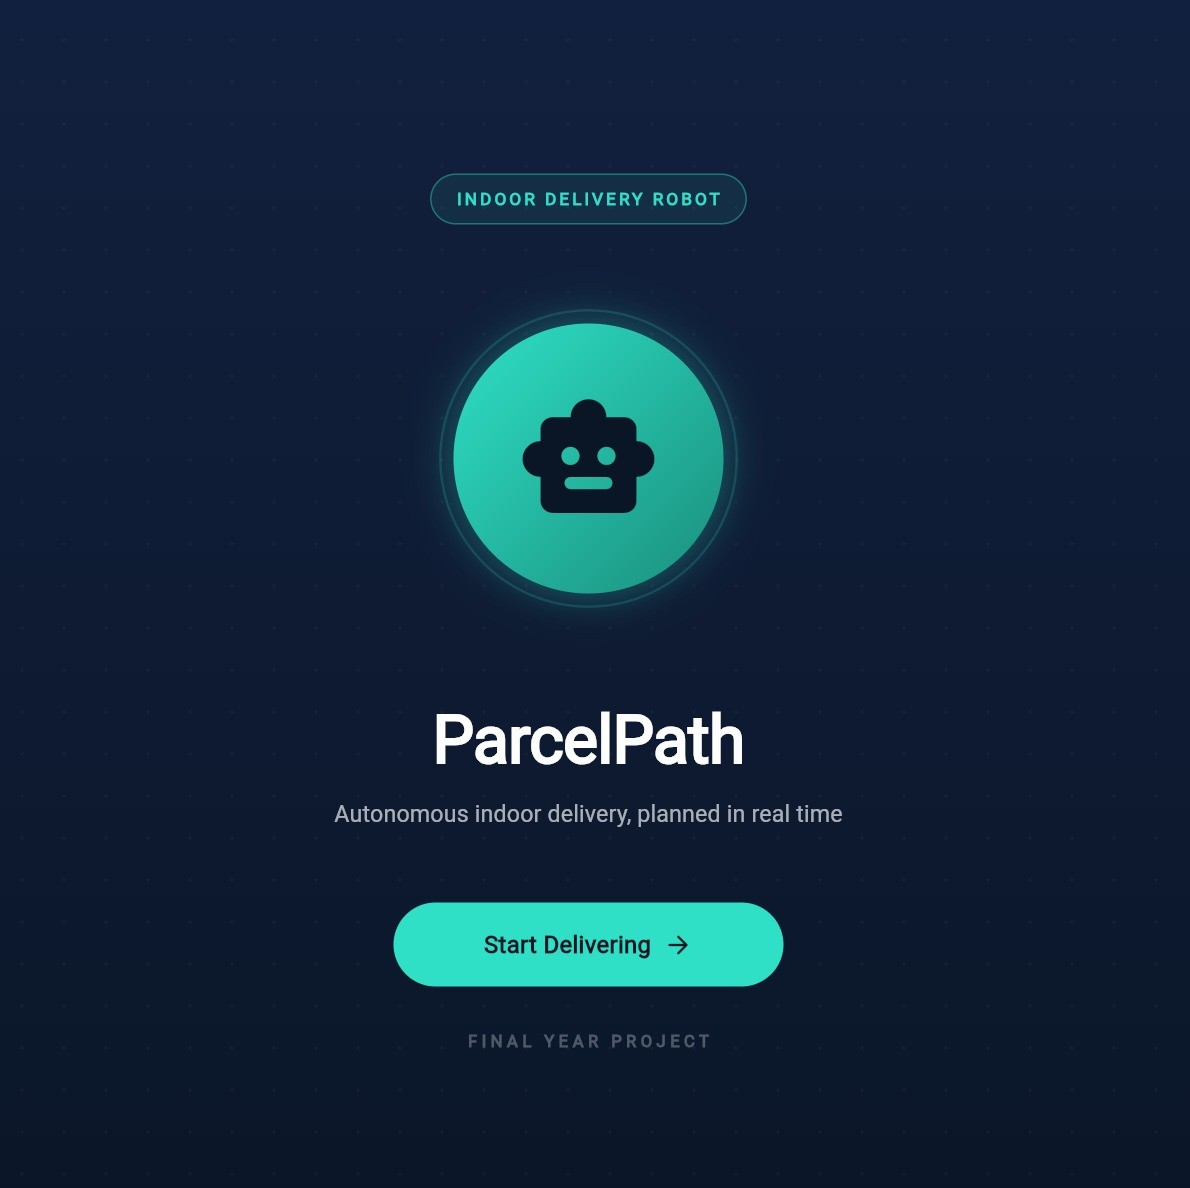
\includegraphics[width=0.5\textwidth]{starting_screen.jpeg}
	\caption{starting screen of the ParcelPath web application}
	\label{fig:starting_screen}
\end{figure}

The starting screen (figure~\ref{fig:starting_screen}) welcomes the user to the system in the name of “Indoor Delivery Robot” and presents the name ParcelPath with the tagline: “Autonomous indoor delivery, planned in real time”. The "Start Delivering" button takes the user forward in the authentication process.

On returning users, the system redirects them to the login screen as shown in Figure~\ref{fig:login} and requires them to log in with their registered email and password to gain access to the delivery portal, while in case of a new user, he is redirected to sign up page as shown in Figure~\ref{fig:signup} where he enters his details such as full name, registered email and password to sign up.


\begin{figure}[H]
	\centering
	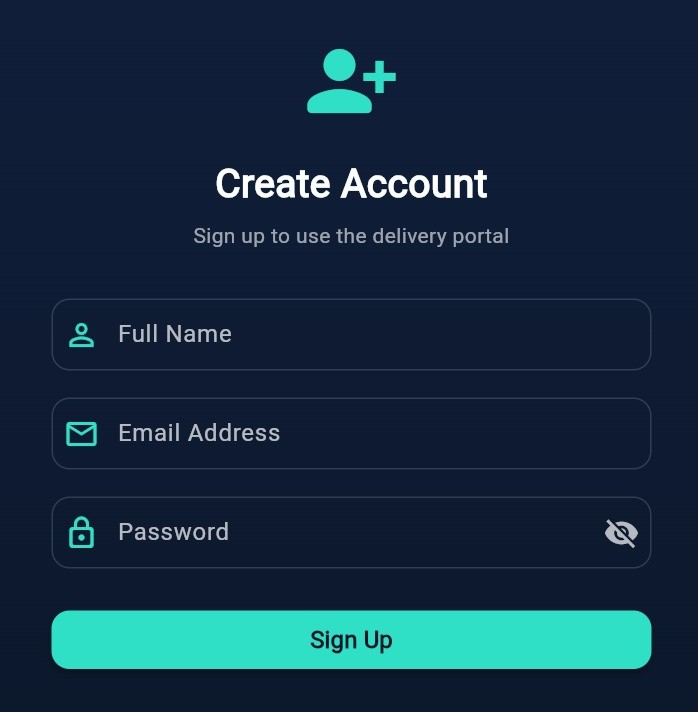
\includegraphics[width=0.5\textwidth]{Sign_up_page.jpeg}
	\caption{Account registration screen for new users}
	\label{fig:signup}
\end{figure}

\begin{figure}[H]
	\centering
	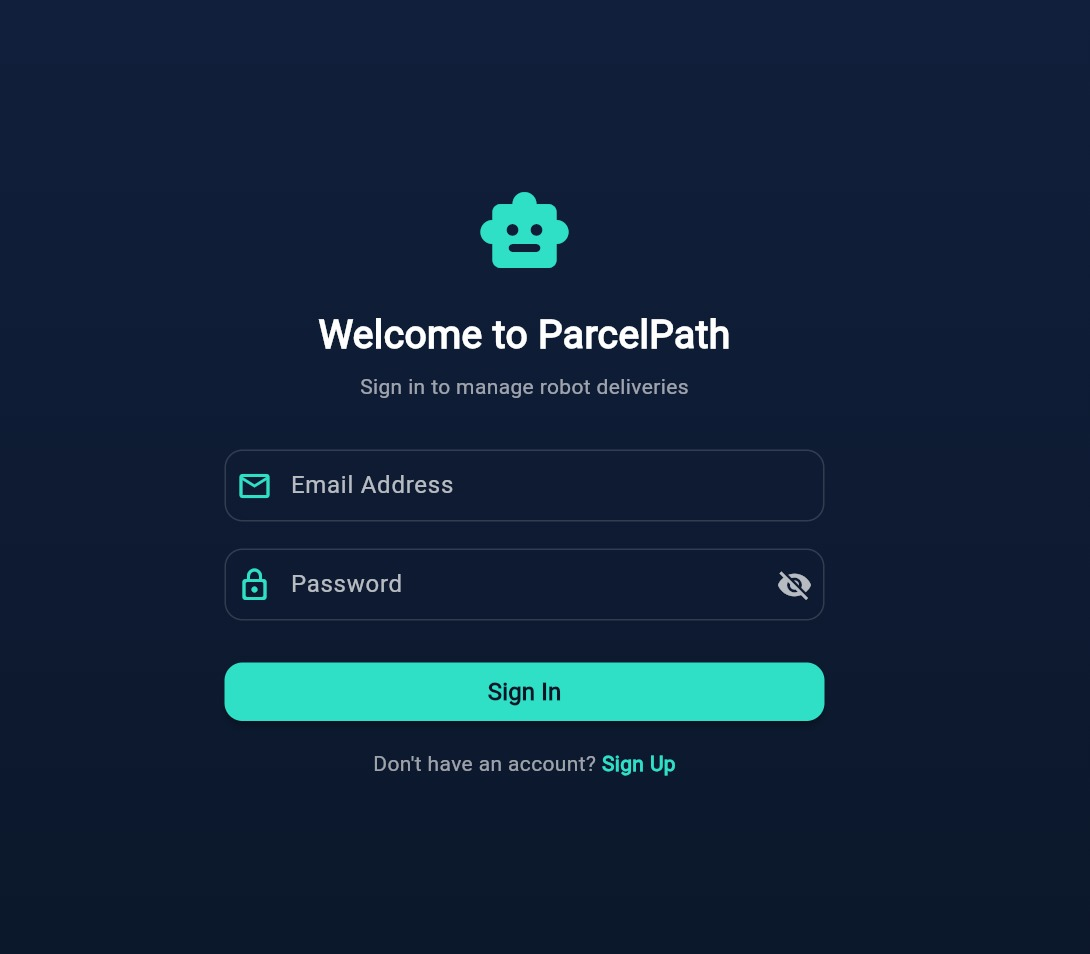
\includegraphics[width=0.5\textwidth]{Login_page.jpeg}
	\caption{Login screen used to authenticate returning users}
	\label{fig:login}
\end{figure}

Both forms have masked password fields with a visibility toggle, and a link to the sign up form for users who haven't already signed up.

\subsection{User Portal and Delivery Requests}

Once authenticated, the user is taken to the User Portal, shown in Figure~\ref{fig:user_portal}, which serves as the main hub for requesting and monitoring deliveries.

\begin{figure}[H]
	\centering
	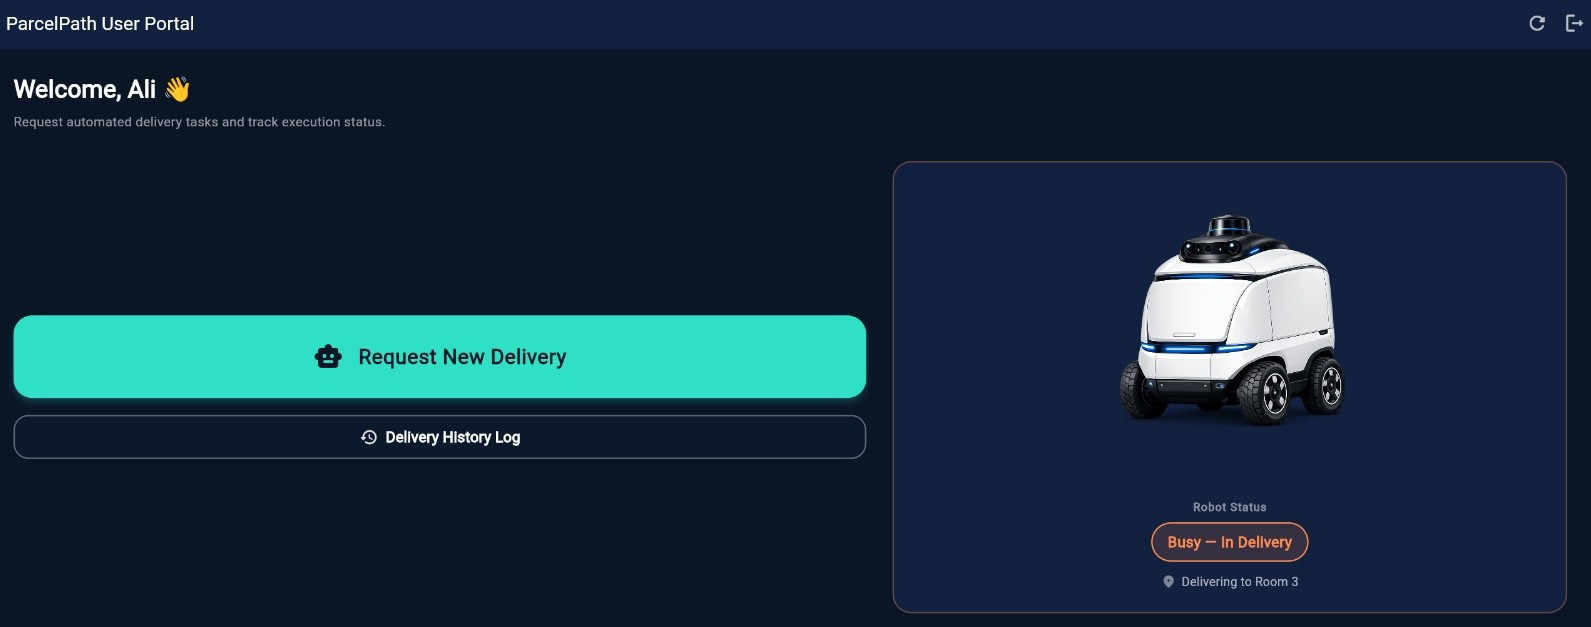
\includegraphics[width=0.9\textwidth]{user_interface.jpeg}
	\caption{User portal showing delivery request options and live robot status}
	\label{fig:user_portal}
\end{figure}

"Request New Delivery," which opens the delivery request form, and "Delivery History Log," which displays previously accomplished deliveries, are the two main activities that the portal offers to the logged-in user after greeting them by name. The robot and its current state—in this case, "Busy - In Delivery"—as well as its current destination are rendered on the status card on the right, providing the user with real-time visibility into robot activity without requiring them to explicitly examine ROS subjects.


Selecting "Request New Delivery" opens the interactive delivery request form shown in Figure~\ref{fig:dispatch_form}.

\begin{figure}[H]
	\centering
	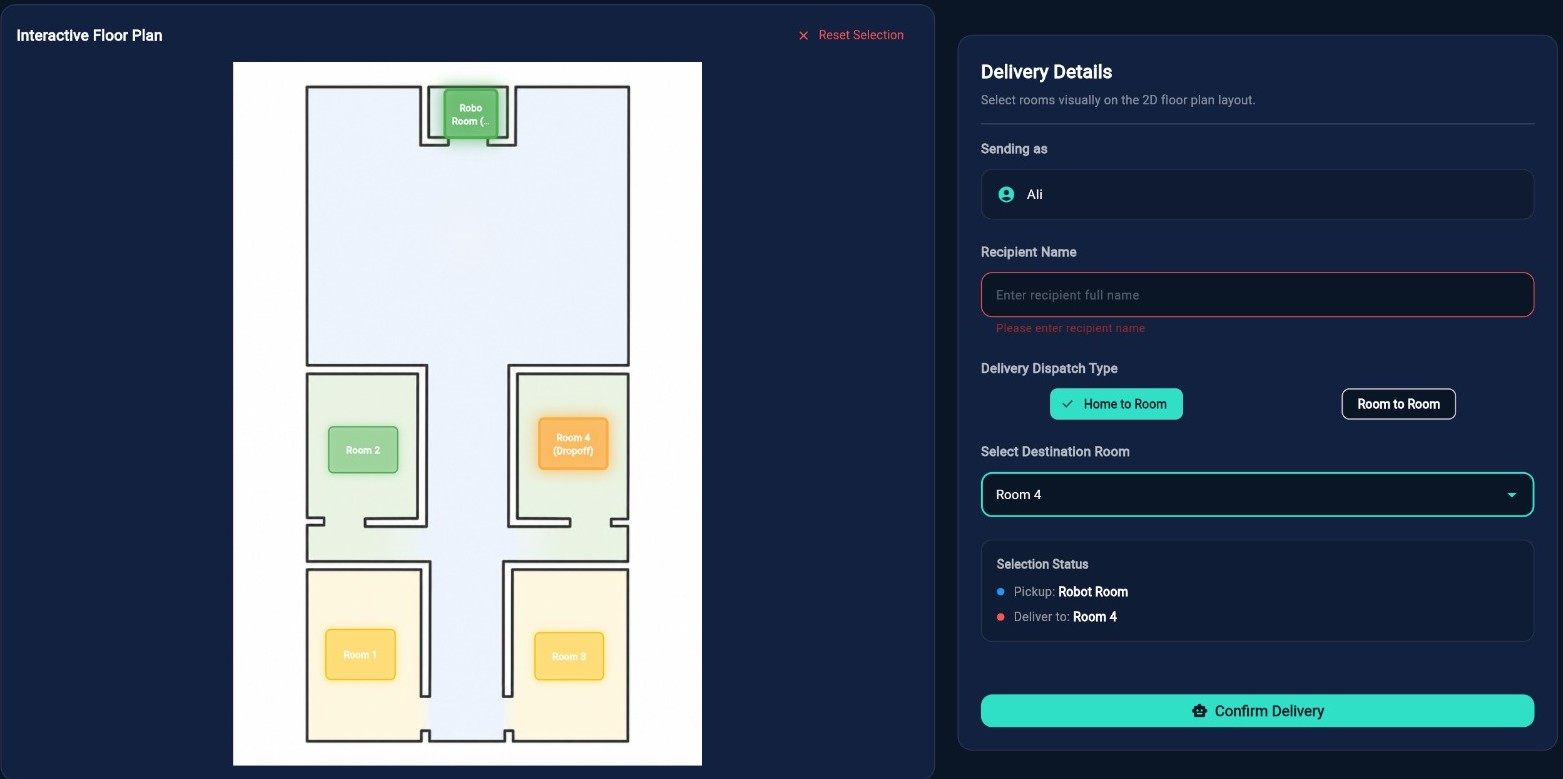
\includegraphics[width=0.95\textwidth]{Dispatching_detail_form.jpeg}
	\caption{Delivery request form with interactive floor-plan room selection}
	\label{fig:dispatch_form}
\end{figure}

Each room is depicted as a selectable colored block in the left panel, which shows the same floor plan used to create the Gazebo world (Figure~\ref{fig:2dmap}). Before the request can be made, the recipient's name must be entered in the Delivery Details panel on the right, which automatically fills in the sender's name from the logged-in account. "Home to Room" or "Room to Room" are the two dispatch kinds that the user can select. The destination can be tapped directly on a room in the floor plan or selected from a dropdown menu. Before the user completes the request with the "Confirm Delivery" button, which transforms the chosen rooms into the matching ROS navigation coordinates and sends the task to the robot, a live "Selection Status" summary verifies the resolved pickup and drop-off rooms.


\subsection{Administrator Operations Hub}

System administrators are directed to a separate Admin Operations Hub, shown in Figure~\ref{fig:admin_hub}, rather than the delivery request screen used by regular users.

\begin{figure}[H]
	\centering
	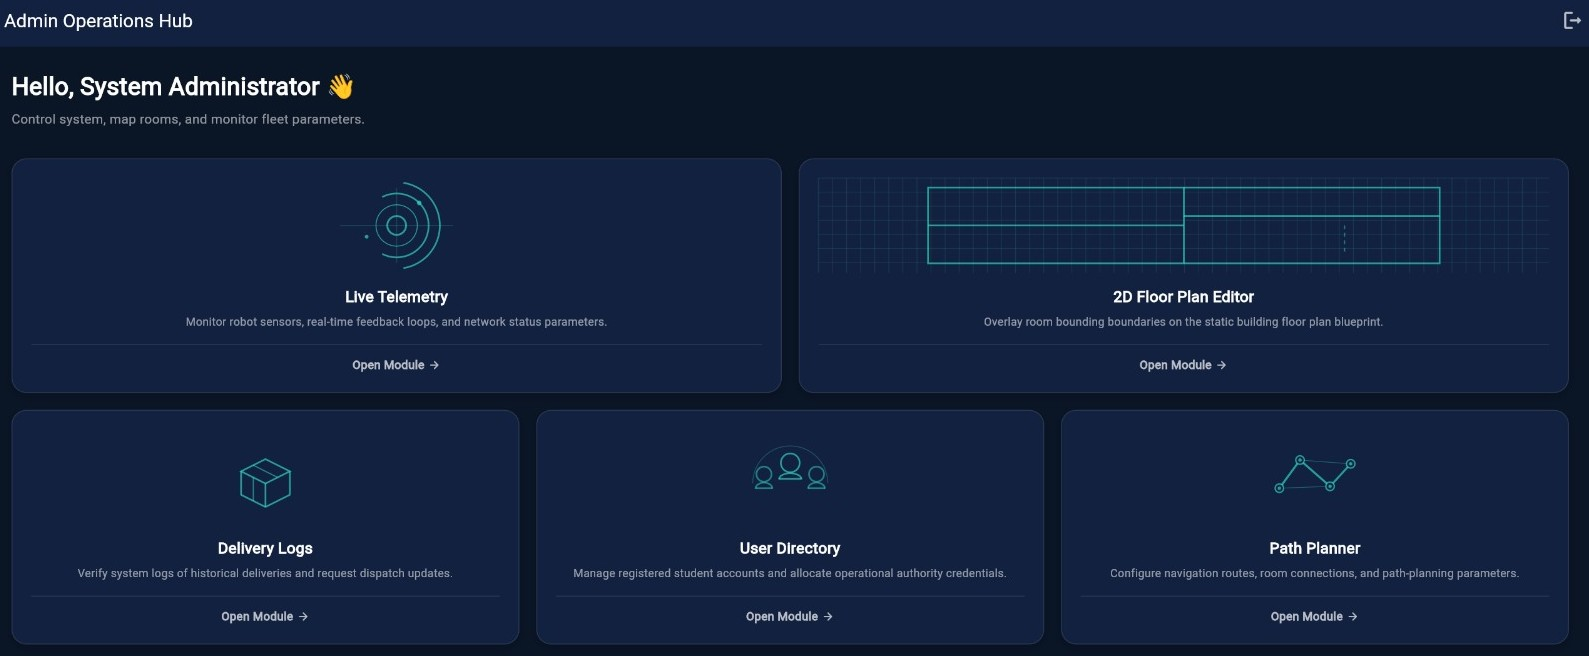
\includegraphics[width=0.95\textwidth]{admin_interface.jpeg}
	\caption{Admin Operations Hub providing access to fleet monitoring and configuration modules}
	\label{fig:admin_hub}
\end{figure}

The hub divides administrative tasks into five modules: the Path Planner, which configures navigation routes, room connections, and planning parameters; the User Directory, which manages registered accounts and access levels; the 2D Floor Plan Editor, which overlays room boundaries on the facility blueprint; Delivery Logs, which examines the historical record of completed and pending deliveries; and Live Telemetry, which monitors robot sensors, feedback loops, and network status in real time. With its own "Open Module" link, each module can be opened separately.


\subsection{2D Floor Plan Editor}

The 2D Floor Plan Editor, opened from the Admin Operations Hub, allows the administrator to map each physical room to its corresponding coordinates in the robot's navigation frame, so that room selections made in the user-facing delivery form (Figure~\ref{fig:dispatch_form}) resolve to valid goal poses for the robot.

\begin{figure}[H]
	\centering
	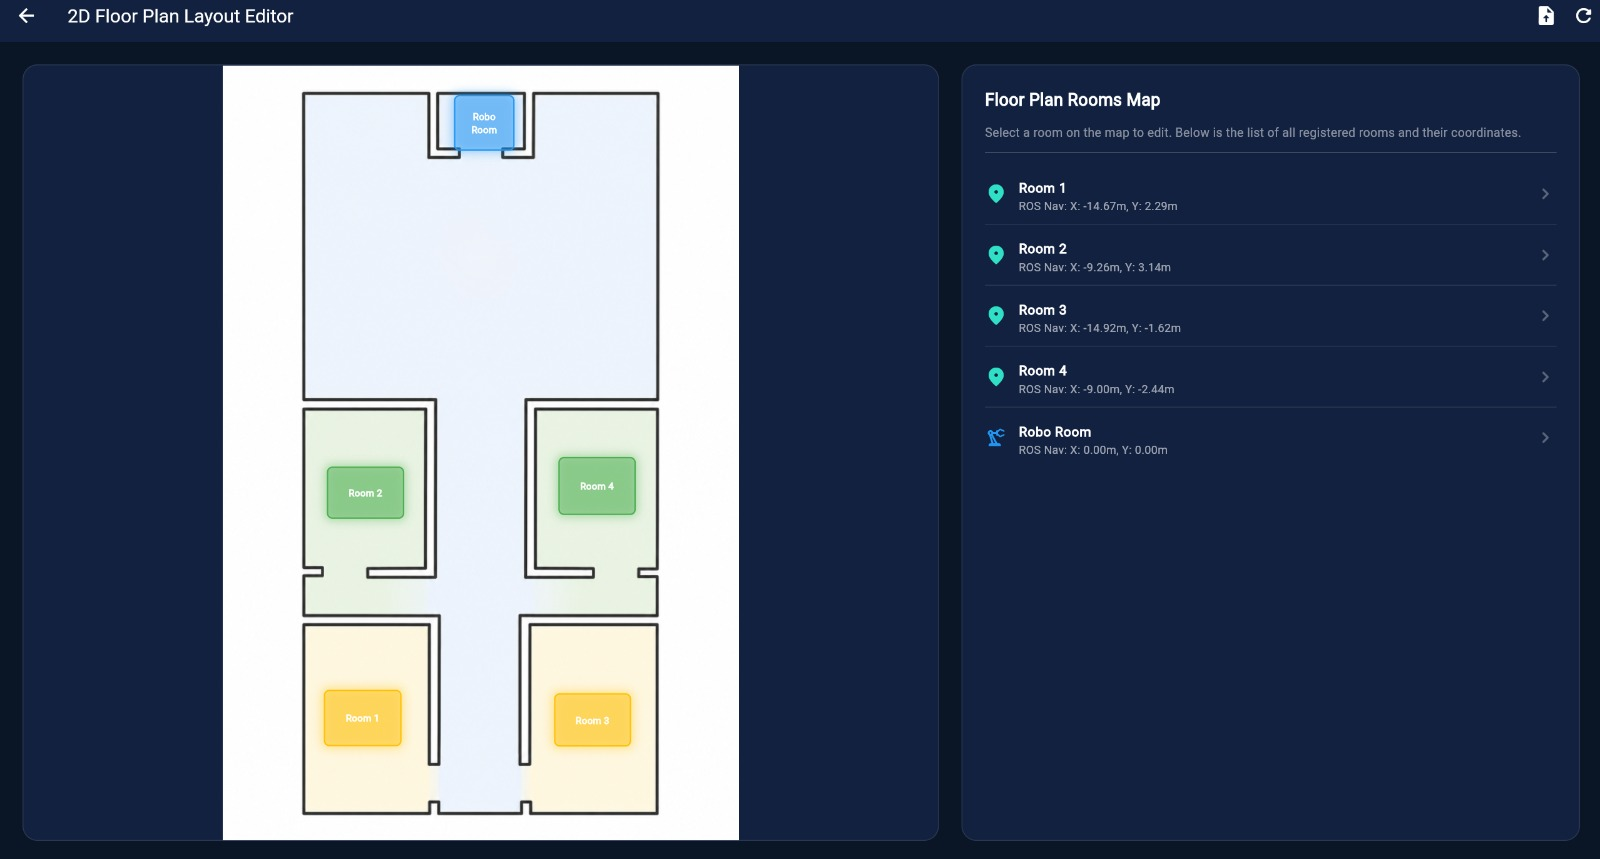
\includegraphics[width=0.95\textwidth]{2d_plan_editor_opt_from_admin_interface.jpeg}
	\caption{2D Floor Plan Layout Editor listing all registered rooms with their ROS navigation coordinates}
	\label{fig:plan_editor_list}
\end{figure}

Figure~\ref{fig:plan_editor_list} shows the floor plan on the left, with each room drawn as a coloured block, alongside a "Floor Plan Rooms Map" list on the right enumerating every registered room, including the robot's own home position ("Robo Room"), together with its stored ROS navigation X and Y coordinates in metres. Selecting a room from this list, or tapping it directly on the map, opens the corresponding editing controls.

\begin{figure}[H]
	\centering
	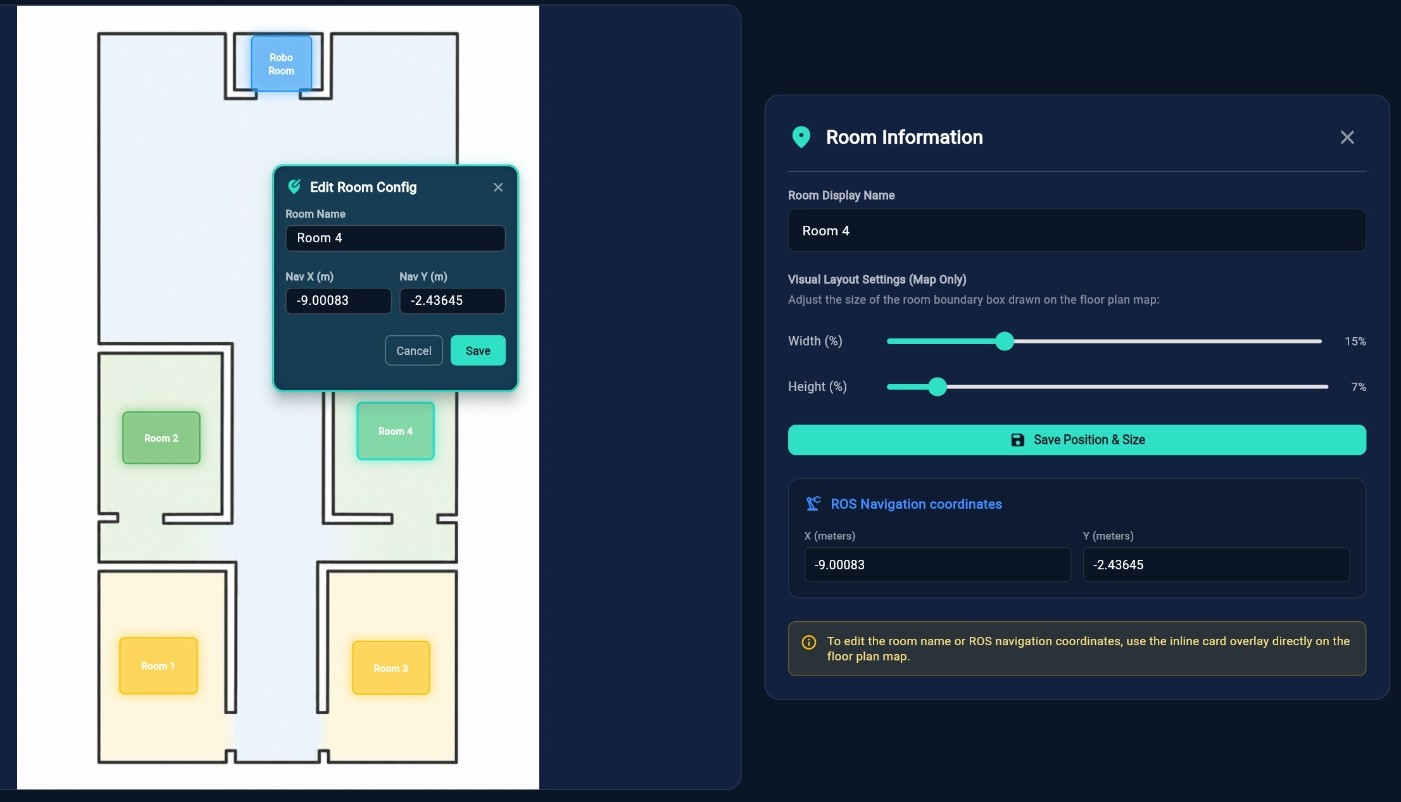
\includegraphics[width=0.95\textwidth]{2d_plan_editor_options_for_changing_sch_as_coordinates.jpeg}
	\caption{Room configuration panel for editing a room's display name, ROS navigation coordinates, and on-map bounding box}
	\label{fig:plan_editor_edit}
\end{figure}

As shown in Figure~\ref{fig:plan_editor_edit}, selecting a room opens an "Edit Room Config" dialog together with a "Room Information" side panel.The administrator can then change the name of the room, directly enter the X and Y coordinates of navigation in the room, and set the width and height of the bounding box for the room on the visual floor plan using percentage sliders, without altering the navigation coordinates saved in the room. The only information that is saved and restored with the position and size changes is the position of the room that is drawn on the map; the separate "ROS Navigation coordinates" fields allow to use the visual layout and navigation data independently, so that they can be edited separately. This separation enables the on-screen floor plan to be optimised for clarity, without the possibility of unintentionally altering the robot's calibrated delivery points.

% ─────────────────────────────────────────────────────────────────────────────
\subsection{Live Robot Camera Monitoring}

The administrator interface also allows the administrator to configure the navigation environment, and to get a live video stream from the robot's onboard RGB camera in the case of a delivery mission being executed. This feature allows the operators to visualize the robot context in real time without having to access ROS~2 visualization tools directly.

The video feed allows the administrator to see the movements of the robot and any pedestrians or other moving obstacles, and the progress of the delivery task. The solution allows the live video stream to be immediately integrated into the web application, enhancing situational awareness and offering a viable tool for controlling the robot remotely.

\begin{figure}[H]
	\centering
	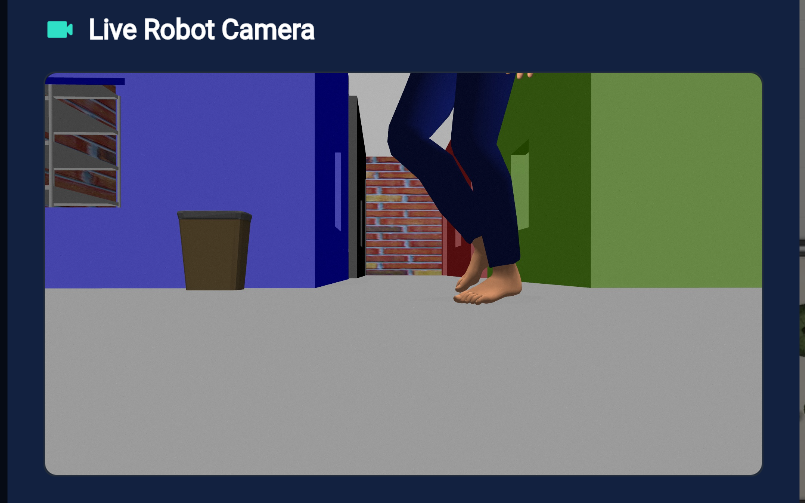
\includegraphics[width=0.6\textwidth]{live_robot_camera.png}
	\caption{Live robot camera feed displayed through the administrator interface.}
	\label{fig:live_camera}
\end{figure}

The live RGB camera feed received by the robot during its navigation in the delivery environment is shown in figure~\ref{fig:live_camera}. The administrator can see what the robot is doing in the current area, such as corridors, room entry points and other people who are close by the robot so that the delivery process can be constantly monitored. This ability adds an extra layer of operational awareness and helps in verifying safe autonomous navigation throughout the mission.

\section{Phase 5: ROS 2 and Gazebo Simulation Results}

In the last phase, all the previously validated planning and control algorithms were transferred to a completely integrated ROS~2 and Gazebo simulation. This milestone is the first time that we have successfully implemented the full stack of SLAM, simulated LiDAR and camera sensing, and our own IA*-based global planner, pruner, spline smoother and MPC controller pipeline in a custom ROS~2 node, and autonomously executed parcel delivery missions within a custom multi-room indoor world, without using any navigation planner.

\subsection{Custom Multi-Room Delivery Environment}
A realistic multi-room environment, like an office floor, was replicated in Gazebo, an indoor world created specifically for the project. The environment is made up of five different rooms, each given a colour coding red, green, grey, blue and teal with a central corridor linking all the rooms and an outer boundary wall. Each room has only one portal to the corridor and the robot can only enter the room through one protected portal, as in a real indoor delivery.\begin{figure}[H]
	\centering
	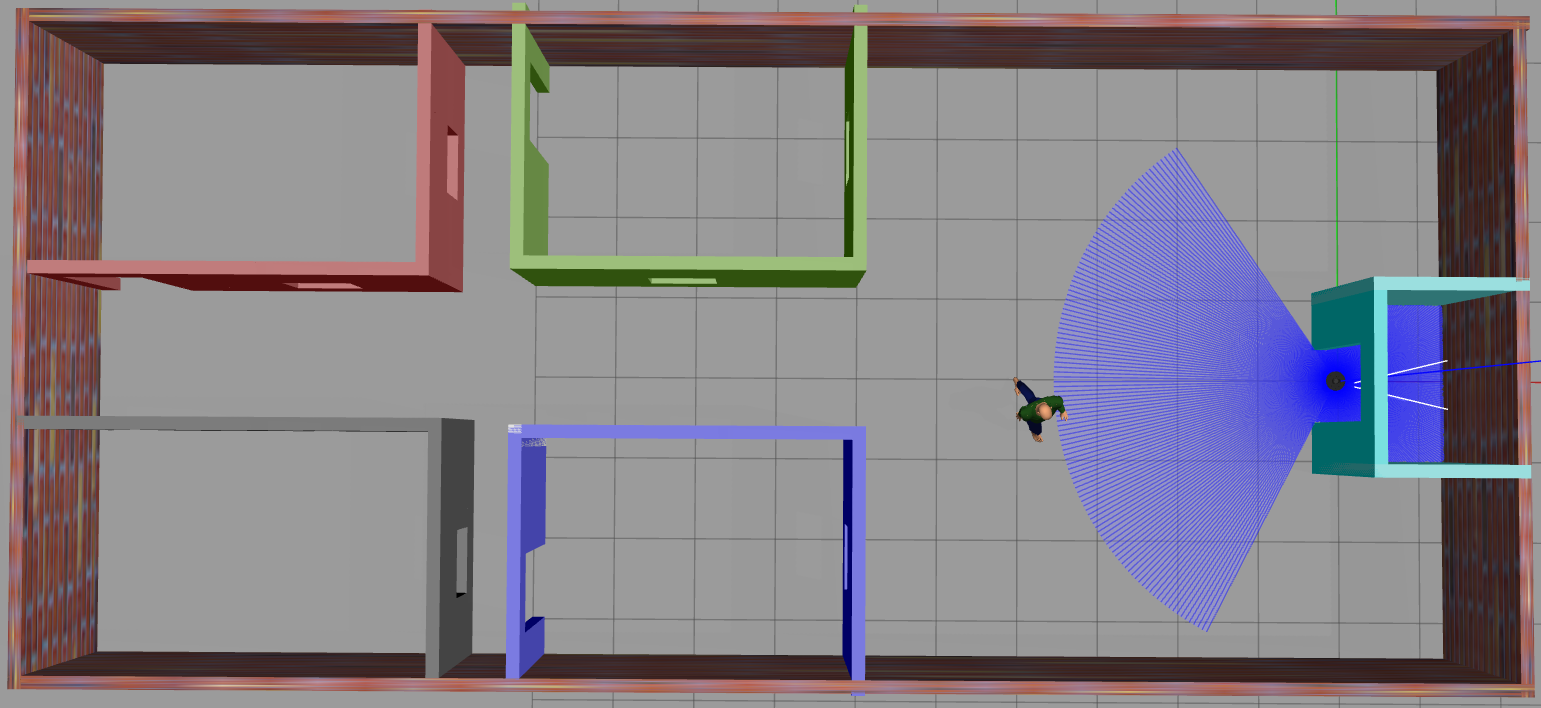
\includegraphics[width=0.9\textwidth]{gazebo_world.png}
	\caption{view of the multi-room Gazebo delivery environment}
	\label{fig:gazebo_world}
\end{figure}

Figure~\ref{fig:gazebo_world} shows the base layout viewed from above. The robot's 360-degree LiDAR footprint appears as the blue fan-shaped region, confirming that the simulated scanner correctly registers the surrounding walls and corridor space. A walking human actor near the robot was scripted to move across the corridor as an unpredictable dynamic obstacle.

The rooms were further populated with furniture models, including sofas, chairs, desks, filing cabinets, a vending machine, and a parked utility vehicle outside the building. This furnished world, shown in Figure~\ref{fig:gazebo_furnished}, was used for all subsequent trials, since it adds static clutter that the planners must account for.

\begin{figure}[H]
	\centering
	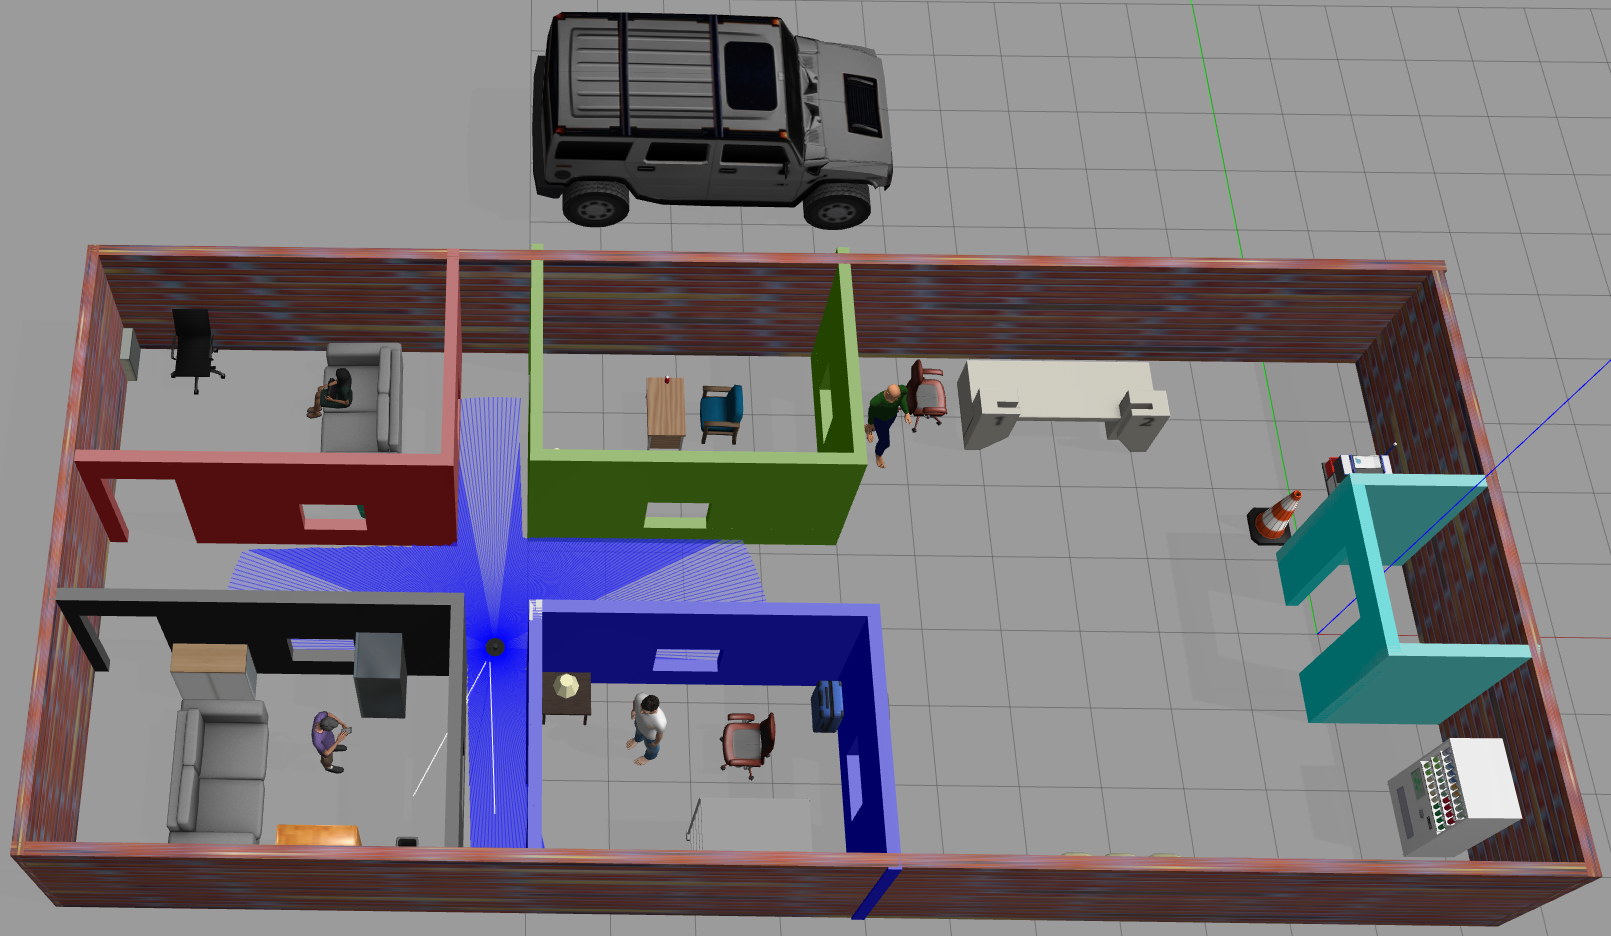
\includegraphics[width=0.9\textwidth]{In_middle_of_delivery.png}
	\caption{Isometric view of the fully furnished delivery environment}
	\label{fig:gazebo_furnished}
\end{figure}

\subsection{Reference Floor Plan}

The room arrangement, door locations, and corridor widths were planned using a simplified two-dimensional floor plan prior to the construction of the world in Gazebo. The zoning is color-coded in this schematic, which is displayed in Figure~\ref{fig:2dmap}. Yellow denotes the two enclosed side rooms, green the two mid-corridor rooms, and blue the open corridor and delivery area that connects them. When positioning walls and doors in the Gazebo world files, it served as a direct reference.


\begin{figure}[H]
	\centering
	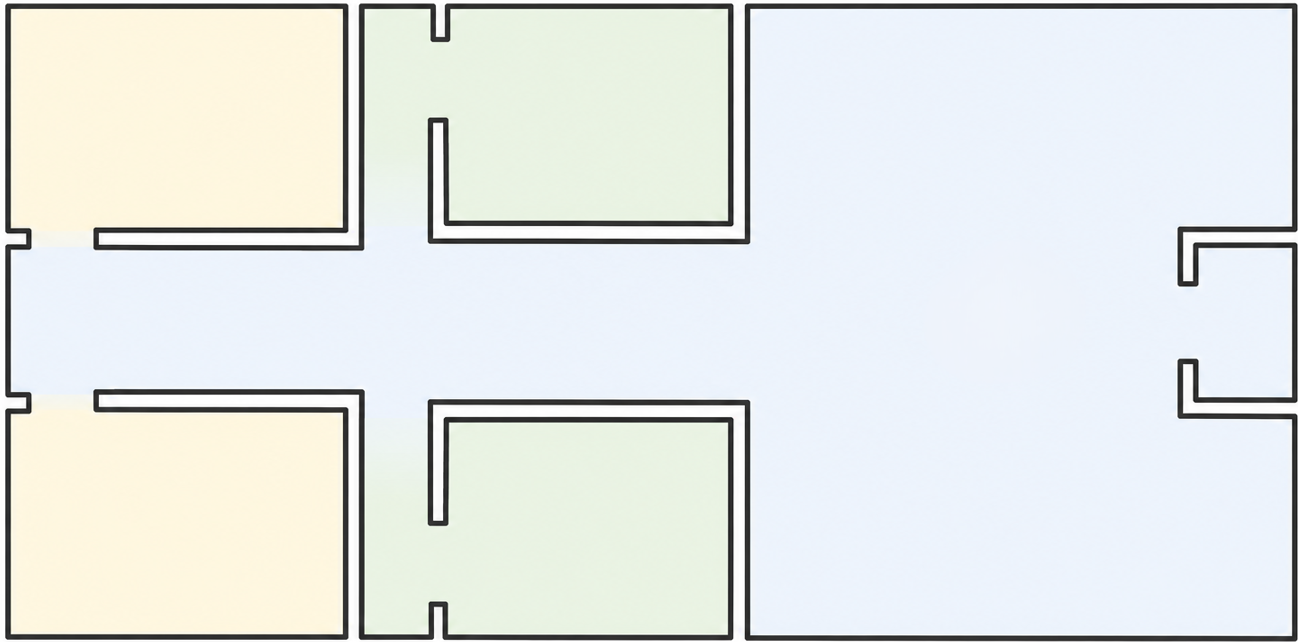
\includegraphics[width=0.9\textwidth]{2d_map_of_world.png}
	\caption{Reference 2D floor plan used to design the room layout of the Gazebo world}
	\label{fig:2dmap}
\end{figure}

\subsection{SLAM-Based Occupancy Mapping}

With the world constructed, the robot was driven through the environment using ROS~2's SLAM stack, based on LiDAR scan matching, to autonomously build a 2D occupancy grid map. The resulting map, shown in Figure~\ref{fig:slam}, closely mirrors the reference floor plan of Figure~\ref{fig:2dmap}, correctly reconstructing every wall, doorway, and room boundary from raw sensor data. The small outlines inside each room correspond to the furniture pieces, confirming the LiDAR resolves obstacles with enough detail for downstream planning, and the red marker denotes the robot's estimated pose.

\begin{figure}[H]
	\centering
	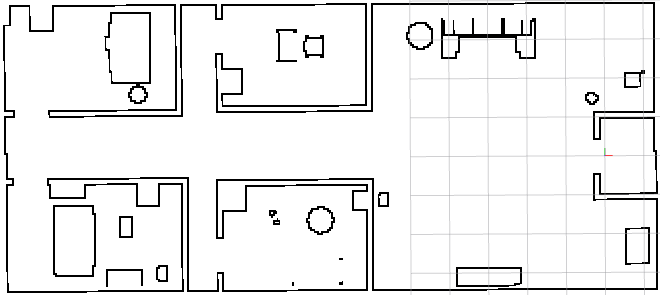
\includegraphics[width=0.85\textwidth]{Slam_output_of_world_with_objects.png}
	\caption{Occupancy grid map generated through SLAM}
	\label{fig:slam}
\end{figure}

This SLAM-generated map was saved and supplied directly to our own path-planning nodes as the static map, on top of which the same obstacle inflation strategy developed in Phase 3 was applied to build the inflated planning map used for the global path search.


\subsection{Path Planning and Smoothing in RViz}



To validate the planning and smoothing pipeline under realistic conditions, a test was conducted in a cluttered obstacle environment. The generated global path was inflated around obstacle boundaries to maintain a safe clearance margin, after which the raw IA* path was refined using the pruning and PSO-based smoothing stages. The pipeline then generated a planning map (Figure~\ref{fig:planning_smoothing_test}) that was inflated, a initial planned path, and a final smoothed planning path while navigating through the obstacle dense environment.

\begin{figure}[H]
	\centering
	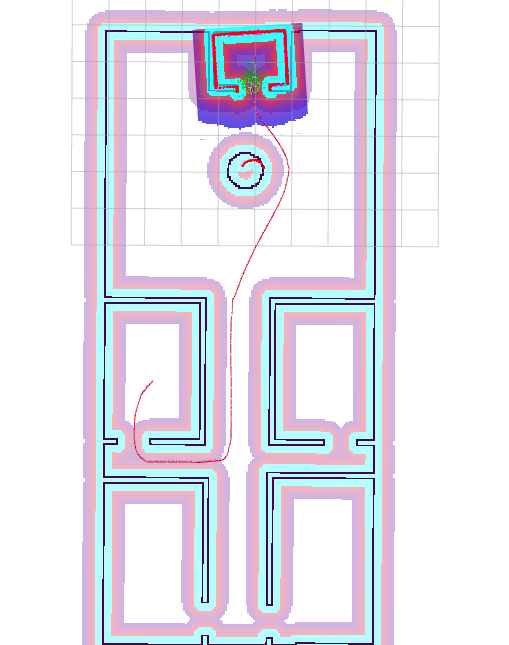
\includegraphics[width=0.6\textwidth]{di.png}
	\caption{Path Planning and Smoothing Test Under an Obstacle Environment}
	\label{fig:planning_smoothing_test}
\end{figure}

The results show that the planner is able to generate the route that does not collide with the obstacles while maintaining the inflated safety margins and the smoothing stage results in a continuous trajectory that is suitable for the motion controller.
Once localized within the SLAM-generated map, the robot was assigned a pickup goal, and the resulting inflated planning map, planned path, and smoothing behaviour produced by our own IA*, pruning, and spline-smoothing pipeline were visualized in RViz. Figure~\ref{fig:rviz_planning} shows the obstacle-inflated map overlaid on the static map, where the light pink region is the inflation buffer and the cyan outline marks the true obstacle boundaries. The red trace shows the path generated by our global planner and refined by the smoothing stage, while the small spiral near the goal is a brief in-place recovery rotation performed by our MPC controller to correct heading before the final approach.

\begin{figure}[H]
	\centering
	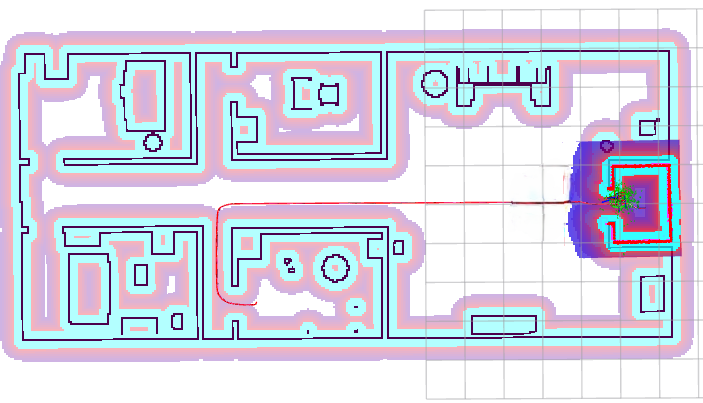
\includegraphics[width=0.85\textwidth]{rviz_p.png}
	\caption{RViz visualization of planned path, and smoothing behaviour produced by custom path-planning pipeline while the robot approaches the pickup location}
	\label{fig:rviz_planning}
\end{figure}

The pruning and smoothing pipeline validated earlier in Section 5.1, Step 4, carried over correctly into the full ROS~2 integration, producing trajectories that remain collision-free and remain practically followable by our own MPC controller, as confirmed by the clean, continuous curvature of the path through the narrow corridor sections.


\subsection{Dynamic Obstacle Avoidance}
A human actor was given instructions to stroll across the robot's intended delivery route while it was navigating toward its destination in order to assess the robustness of the suggested navigation framework in dynamic interior situations.
The experiment is presented in a top-down view in Figure~\ref{fig:person_avoidance} where the robot's LiDAR continually scans the environment around him and detects the moving pedestrian when it enters into the environment's sensing range.

The robot first follows the globally optimized path which was computed using the A* algorithm, then the path is pruned and then smoothed using PSO. Upon detecting the pedestrian, the MPPI (Model Predictive Path Integral) controller predicted multiple short-horizon feasible trajectories in real-time based on the measured LiDAR data, while accounting for obstacle clearance, path tracking precision and smoothness of the motion. The controller chose the path of the lowest cost to avoid collisions, with the robot temporarily off of the path of the original global path, but still navigating safely around the moving obstacle.

Once the pedestrian was out of the robot's way, the obstacle was deleted from the local cost map and the MPPI controller took the robot back to the smoothed global trajectory. The global path was valid and no global replanning was needed. With this local trajectory optimization, collision-free, smooth, continuous navigation towards the delivery target was achieved without any manual inputs.

\begin{figure}[H]
	\centering
	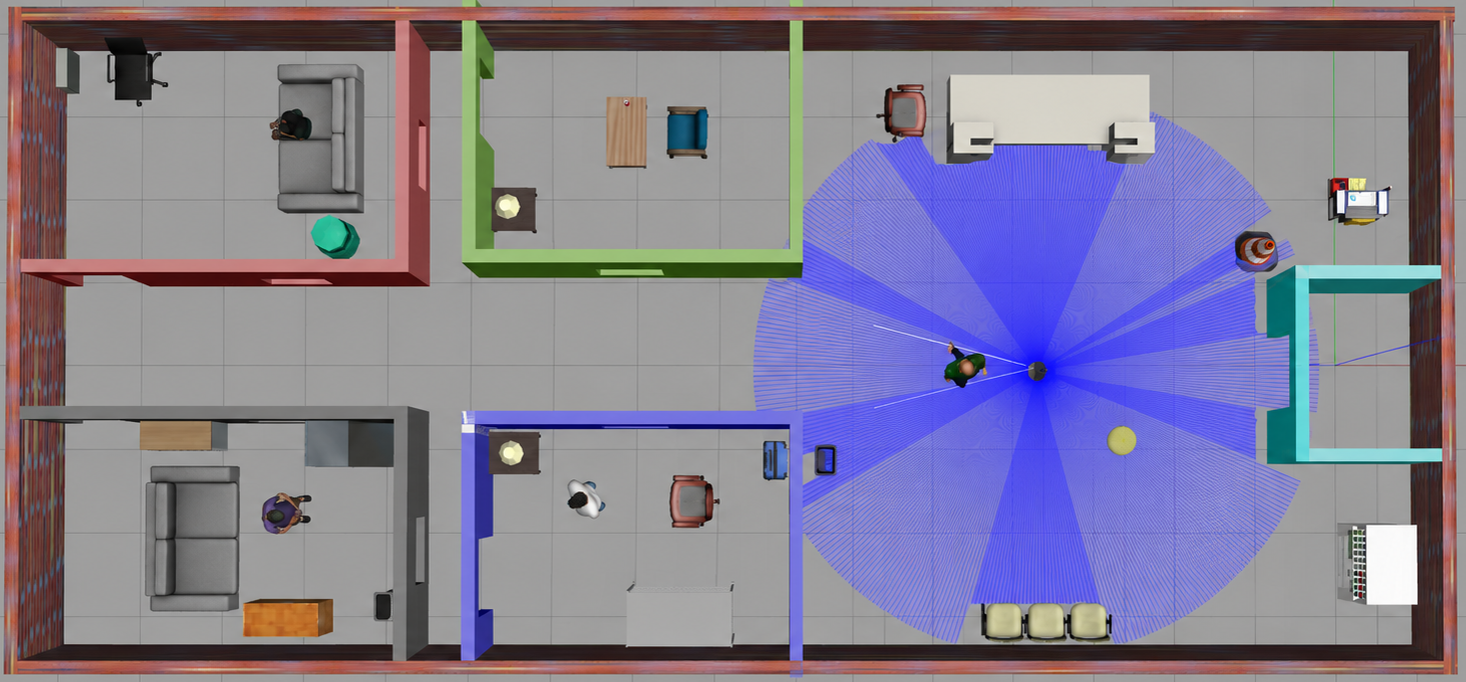
\includegraphics[width=0.9\textwidth]{person_avoidance_during_delivery.png}
	\caption{Robot detecting and safely avoiding a moving pedestrian during a parcel delivery task.}\label{fig:person_avoidance}
\end{figure}
\subsection{Arrival at the Delivery Point}

Once the robot reaches its delivery room, it is seen in Figure~\ref{fig:delivery_point}. The robot has stopped at the designated goal location once it enters the authorized drop-off area. The objective coordinate (obtained from the web interface) was successfully converted into the map frame, and the robot went through the environment safely, without colliding with any obstacles, as evidenced by the successful arrival.

\begin{figure}[H]
	\centering
	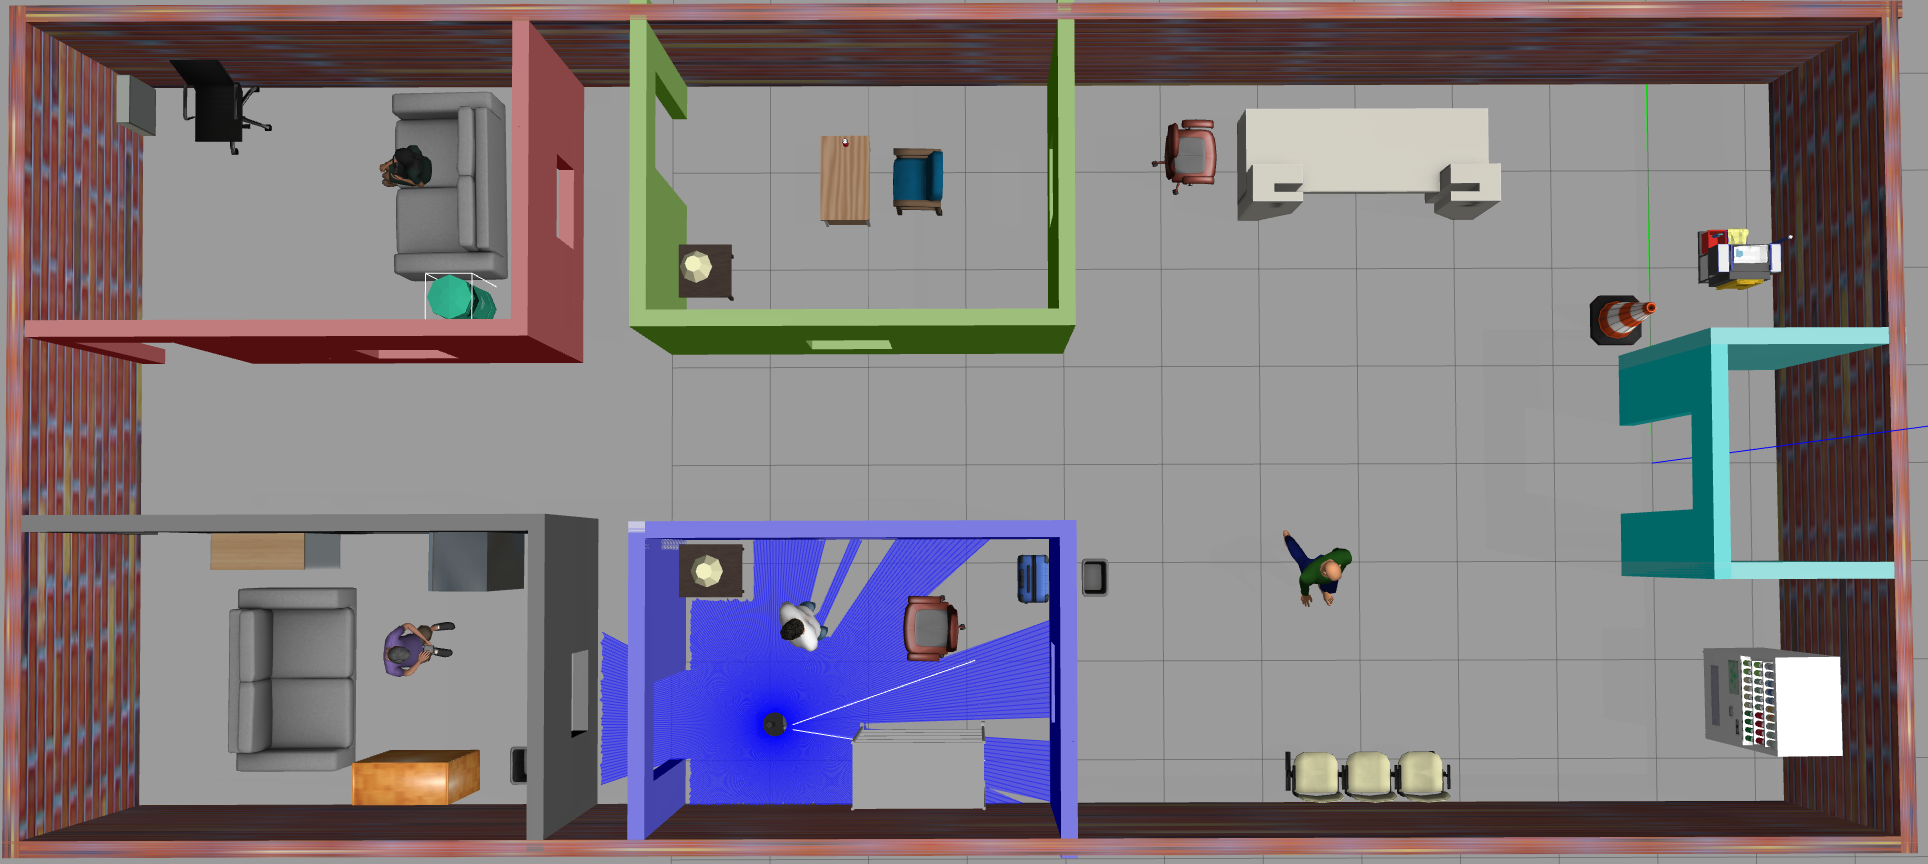
\includegraphics[width=0.9\textwidth]{gazebo_marking_robot_at_delivery_point.png}
	\caption{Robot arriving at the designated delivery point inside the drop-off room}
	\label{fig:delivery_point}
\end{figure}

\subsection{Complete Delivery Mission}

Lastly, the RViz visualization following a successful end-to-end parcel delivery mission is shown in Figure~\ref{fig:rviz_complete}. While the MPPI controller continually carried out local trajectory optimization to safely avoid dynamic impediments as they were met, the robot began at the pickup site and followed the globally optimized trajectory created using the A* algorithm, route trimming, and PSO-based path smoothing. The trajectory that is shown shows the entire path that the robot took, ending at the specified delivery location. The mission's successful conclusion shows how global path planning, path optimization, local obstacle avoidance, and autonomous navigation may be seamlessly integrated to enable dependable end-to-end parcel delivery without the need for human intervention.

\begin{figure}[H]
	\centering
	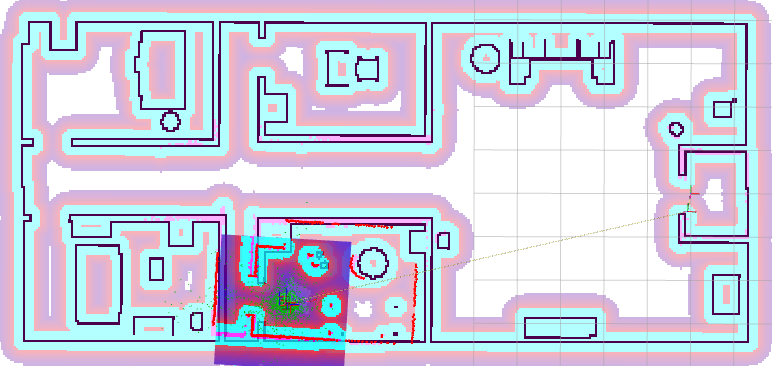
\includegraphics[width=0.85\textwidth]{rviz_showing_complete_delivery.png}
	\caption{RViz visualization confirming successful completion of the full delivery mission from pickup to drop-off}
	\label{fig:rviz_complete}
\end{figure}

Together, these results demonstrate the successful integration of the proposed navigation framework, consisting of SLAM-based mapping, obstacle inflation, A*-based global path planning, path pruning, PSO-based path smoothing, MPPI-based local trajectory optimization, and LiDAR-based dynamic obstacle avoidance. In the ROS~2 and Gazebo environments, the suggested system successfully completed end-to-end parcel delivery missions, precisely moving across several rooms while securely avoiding both static and dynamic impediments. These outcomes confirm that the suggested navigation architecture for autonomous interior parcel delivery is reliable and efficient.


\section{Limitations of the Working Prototype}

The functioning prototype has a number of drawbacks, despite the suggested navigation framework's dependable performance in the ROS~2 and Gazebo simulations. Since the complete system was only tested in simulation, it hasn't been verified on a real robot with sensors, motors, and network hardware, where performance could be impacted by noise, latency, and mechanical flaws. The robustness of dynamic obstacle avoidance in busier, more chaotic contexts is yet unknown because it was evaluated against a single planned pedestrian rather than several, erratic human movements. Additionally, because the system depends on a manually specified floor plan and a pre-built SLAM map, it is currently unable to automatically adjust to changes in the environment, such as rearranging rooms or moving furniture.
Additionally, the existing design only allows one robot at a time and lacks a system for managing shared passageways or coordinating several robots. Lastly, as they are outside the purview of a simulation-based prototype, issues like battery life, charging, and long-term autonomous operation were not covered.

\section{Challenges Faced}

Several technical difficulties arose during the implementation and integration of several software components during the autonomous parcel delivery system's development. Before a solid and dependable system was created, these difficulties necessitated a great deal of debugging, parameter adjusting, and iterative testing.\begin{itemize}
     \item \textbf{Obstacle Collision During Path Planning:}
	In the initial stages of path planning some projected paths were too close to the obstacles and could lead to a potential collision. Obstacle inflation and definition of safe margins allowed the robot to safely navigate to the destination.


\item \textbf{Path Smoothing Issues:}
The paths generated by the Improved A* algorithm were not only not collision free, but had sharp turns that were difficult to follow smoothly by the robot. The cubic spline interpolation was used to produce smoother curves and maintain a safe distance from obstructions. There was a few iterations to get the balance between path accuracy and smoothness right.

\item \textbf{Gazebo Installation and Simulation Setup:}
The setup of Gazebo simulation environment was one of the initial challenges faced by the project. In rare cases, there were rendering and resources setting issues, which lead to black screen or world not loading. These problems were resolved by selecting the right rendering engine, ensuring the paths for resources were set up correctly, and installing the dependencies.


\item \textbf{Custom World Development:}
It was necessary to build rooms, hallways, furniture, doors, and moving human actors while making sure the robot had enough area to move about securely in order to create a realistic indoor setting. A series of changes in the size of the items, collision properties, and placement of the models was made until a steady simulation environment was achieved.

\item \textbf{Motion Controller (MPC) Tuning:}
The first problem with this robot is that it was initially having trouble following the paths accurately generated by the global planner. To enable the robot to follow the intended course in different scenarios, the MPC controller required fine tuning of prediction horizons, weights on the control and velocity limitations.


\item \textbf{ROS~2 and Web Application Integration:}
A major challenge was to integrate the Flutter web application into the ROS~2 navigation system. Reliable communication between the Flutter frontend, the Flask backend and the ROS~2 nodes was necessary to send delivery requests, receive robot status information and accurately display real information.


\item \textbf{Package Dependency Conflicts:}
During installation and upgrades, the project's use of multiple ROS~2 packages and third-party libraries occasionally resulted in dependency conflicts. Installing suitable package versions and recreating the workspace as needed fixed these problems.


\item \textbf{Launch File Configuration:}
The system became more complicated due to the need to manage several launch files for Gazebo, SLAM Toolbox, Nav2, the Flask backend, and custom ROS~2 nodes. To make sure that every component began in the right order and functioned as intended, careful planning and frequent testing were necessary.

\item \textbf{System Integration and Testing:}
Integrating all of the system's components path planning, motion control, SLAM, Gazebo, ROS~2, the Flask backend, and the Flutter web application—into a single functional system was the last obstacle. To ensure that the robot could successfully fulfill delivery missions from beginning to end and that all modules communicated appropriately, extensive testing was conducted.


\end{itemize}

Despite these difficulties, a fully integrated autonomous package delivery system with dependable navigation, obstacle avoidance, and real-time user engagement via the web application was produced through constant debugging, parameter tuning, and repetitive testing.

% ══════════════════════════════════════════════════════════════════════════════

\section{Summary}
The design, execution, and assessment of the suggested Autonomous Parcel Delivery System were covered in this chapter through a number of progressive development phases. When the A* algorithm was originally used for global path planning, it produced paths inside the occupancy grid map that were free of collisions. To create shorter, smoother, and robot-friendly trajectories appropriate for autonomous navigation, path trimming and PSO-based smoothing were then used.Obstacle inflation ensured safe planning around static impediments, and a web-based interface was created to allow users to designate pickup and delivery locations.An MPPI controller was specially used to avoid dynamic impediments by carrying out real-time local trajectory optimization based on LiDAR readings, while an MPC controller precisely followed the optimized global trajectory for path execution.
Ultimately, these elements were combined to create a realistic multi-room delivery scenario with pedestrians traveling across the ROS~2 and Gazebo simulation environments. The TurtleBot3 successfully produced a SLAM map, streamed real-time sensor data, planned and optimized collision-free routes, used the MPPI controller to avoid dynamic obstacles, and finished delivery tasks from pickup to drop-off. The results justify the effectiveness and reliability of the proposed navigation system for autonomous interior package delivery.
